% Options for packages loaded elsewhere
\PassOptionsToPackage{unicode}{hyperref}
\PassOptionsToPackage{hyphens}{url}
\PassOptionsToPackage{dvipsnames,svgnames,x11names}{xcolor}
\documentclass[
  ngerman,
  11pt,
  a4paper,
]{article}
\usepackage{xcolor}
\usepackage[margin=23mm]{geometry}
\usepackage{amsmath,amssymb}
\setcounter{secnumdepth}{-\maxdimen} % remove section numbering
\usepackage{iftex}
\ifPDFTeX
  \usepackage[T1]{fontenc}
  \usepackage[utf8]{inputenc}
  \usepackage{textcomp} % provide euro and other symbols
\else % if luatex or xetex
  \usepackage{unicode-math} % this also loads fontspec
  \defaultfontfeatures{Scale=MatchLowercase}
  \defaultfontfeatures[\rmfamily]{Ligatures=TeX,Scale=1}
\fi
\usepackage{lmodern}
\ifPDFTeX\else
  % xetex/luatex font selection
\fi
% Use upquote if available, for straight quotes in verbatim environments
\IfFileExists{upquote.sty}{\usepackage{upquote}}{}
\IfFileExists{microtype.sty}{% use microtype if available
  \usepackage[]{microtype}
  \UseMicrotypeSet[protrusion]{basicmath} % disable protrusion for tt fonts
}{}
\makeatletter
\@ifundefined{KOMAClassName}{% if non-KOMA class
  \IfFileExists{parskip.sty}{%
    \usepackage{parskip}
  }{% else
    \setlength{\parindent}{0pt}
    \setlength{\parskip}{6pt plus 2pt minus 1pt}}
}{% if KOMA class
  \KOMAoptions{parskip=half}}
\makeatother
\usepackage{longtable,booktabs,array}
\newcounter{none} % for unnumbered tables
\usepackage{calc} % for calculating minipage widths
% Correct order of tables after \paragraph or \subparagraph
\usepackage{etoolbox}
\makeatletter
\patchcmd\longtable{\par}{\if@noskipsec\mbox{}\fi\par}{}{}
\makeatother
% Allow footnotes in longtable head/foot
\IfFileExists{footnotehyper.sty}{\usepackage{footnotehyper}}{\usepackage{footnote}}
\makesavenoteenv{longtable}
\usepackage{graphicx}
\makeatletter
\newsavebox\pandoc@box
\newcommand*\pandocbounded[1]{% scales image to fit in text height/width
  \sbox\pandoc@box{#1}%
  \Gscale@div\@tempa{\textheight}{\dimexpr\ht\pandoc@box+\dp\pandoc@box\relax}%
  \Gscale@div\@tempb{\linewidth}{\wd\pandoc@box}%
  \ifdim\@tempb\p@<\@tempa\p@\let\@tempa\@tempb\fi% select the smaller of both
  \ifdim\@tempa\p@<\p@\scalebox{\@tempa}{\usebox\pandoc@box}%
  \else\usebox{\pandoc@box}%
  \fi%
}
% Set default figure placement to htbp
\def\fps@figure{htbp}
\makeatother
\ifLuaTeX
\usepackage[bidi=basic,shorthands=off]{babel}
\else
\usepackage[bidi=default,shorthands=off]{babel}
\fi
\ifLuaTeX
  \usepackage{selnolig} % disable illegal ligatures
\fi
\setlength{\emergencystretch}{3em} % prevent overfull lines
\providecommand{\tightlist}{%
  \setlength{\itemsep}{0pt}\setlength{\parskip}{0pt}}
\usepackage{xcolor}
\definecolor{ink}{HTML}{17344A}
\definecolor{accent}{HTML}{20768A}
\usepackage{microtype}
\usepackage{fancyhdr}
\usepackage{titlesec}
\usepackage{fvextra}
\pagestyle{fancy}
\fancyhf{}
\fancyhead[L]{\small\sffamily TFPT und Universalraum}
\fancyhead[R]{\small\sffamily Forschungssynthese · 15.09.2026}
\fancyfoot[L]{\footnotesize\sffamily Synthese 1.0 · Quellen bis v1.6.7 einschließlich Nachtrag}
\fancyfoot[R]{\thepage}
\setlength{\headheight}{15pt}
\titleformat{\section}{\Large\sffamily\bfseries\color{ink}}{}{0em}{}
\titleformat{\subsection}{\large\sffamily\bfseries\color{ink}}{}{0em}{}
\titleformat{\subsubsection}{\normalsize\sffamily\bfseries\color{ink}}{}{0em}{}
\setlength{\emergencystretch}{3em}
\setlength{\parskip}{5pt}
\setlength{\parindent}{0pt}
\AtBeginEnvironment{longtable}{\small}
\AtBeginDocument{\hypersetup{urlcolor=accent,linkcolor=ink}}
\usepackage{bookmark}
\IfFileExists{xurl.sty}{\usepackage{xurl}}{} % add URL line breaks if available
\urlstyle{same}
\hypersetup{
  pdftitle={TFPT und Universalraum},
  pdfauthor={Forschungssynthese und eigene Herleitungen · erstellt mit Codex},
  pdflang={de-DE},
  colorlinks=true,
  linkcolor={Maroon},
  filecolor={Maroon},
  citecolor={Blue},
  urlcolor={Blue},
  pdfcreator={LaTeX via pandoc}}

\title{TFPT und Universalraum}
\usepackage{etoolbox}
\makeatletter
\providecommand{\subtitle}[1]{% add subtitle to \maketitle
  \apptocmd{\@title}{\par {\large #1 \par}}{}{}
}
\makeatother
\subtitle{Von der markierten Algebra zum gemeinsamen physikalischen
Prozess}
\author{Forschungssynthese und eigene Herleitungen · erstellt mit Codex}
\date{15. September 2026 · Synthese 1.0 · Quellen bis v1.6.7}

\begin{document}
\maketitle

{
\setcounter{tocdepth}{2}
\tableofcontents
}
\section{Zusammenfassung}\label{zusammenfassung}

Die Topological Fixed-Point Theory (TFPT) verbindet eine markierte
algebraische Ausgangsstruktur mit Darstellungen, Gitterdaten und
Kandidaten für physikalische Größen. Der Universalraum bezeichnet das
weitergehende Ziel, Zustände, erlaubte Operationen, Aufzeichnungen und
beobachtbare Entwicklung als Teile einer gemeinsamen Konstruktion zu
verstehen. Die vorliegende Arbeit synthetisiert die bis zum 15.
September 2026 verfügbaren Hauptdokumente, Fortsetzungen und
ausgewählten aktuellen Forschungsartefakte. Sie integriert insbesondere
die beiden verschiedenen v1.6.6-Linien und die neuere v1.6.7 mit ihrer
korrigierten Hamilton-Lanczos-Kette.

Der belastbare mathematische Kern umfasst eine markierte
\(D_5\)--\(A_3\)-Verklebung zu \(E_8\), eine konkrete Darstellung
desselben Gitters in einer Ordnung von \(M_2(\mathbb Q(i))\), endliche
Kontextprozesse, kohärenzverträgliche Aufzeichnungen und eine native
Paarwechselwirkung zwischen 64 Fermion- und 60 Bosonmoden. Für den
ausdrücklich festgelegten nativen Hamiltonoperator liegen Grundzustands-
und Antwortsätze vor. Die jüngste Fortsetzung bestimmt vier
Singulett-Richtungen auf der zweiten Bosonstufe, fünf korrekte
Lanczos-Glieder und zehn Momente der gefüllten Referenz. Sie verschärft
eine Energieobergrenze, ohne die gesamte Bank diagonalisiert zu haben.
Der jüngste Nachtrag identifiziert zusätzlich einen nativen
Rang-60-Kodierer, prüft dessen Grenze bei Modenverlust und klassifiziert
eine Z4-verträgliche Hamiltonfamilie bis zu einer konkreten kanonischen
Reduktion.

Der eigene Beitrag dieser Synthese besteht aus drei Verbindungen.
Erstens wird ein gemeinsamer Prozess durch den positiven Gramkern seiner
zulässigen Operationswörter rekonstruiert; daraus folgt ein präzises
Kriterium dafür, wann zwei vermeintliche Teillösungen tatsächlich
dieselbe Ausführung beschreiben. Zweitens erhält der bisher zusätzliche
Vierzustands-Transfer eine explizite, achtdimensionale Erweiterung mit
einer zweistufigen Ladungsreferenz. Sie erhält die betrachtete
Gesamt-Cartanladung exakt und reproduziert den bekannten Transferblock;
sie beweist nicht die Herkunft dieser Referenz. Drittens werden
Überlappung, dynamische Kompression und Projektorgeometrie
zusammengeführt. Ein bewegter physischer Unterraum kann geometrische
Krümmung tragen, während eine bloße Basisrotation im festen
vollständigen Raum keine erzeugt. Ein konkreter Zweikomponentenzeuge
liefert sowohl Krümmung als auch Zustandsmetrik und eine exakt bezahlte
selektive Schleifenwahrscheinlichkeit.

Diese Ergebnisse liefern einen mathematisch zusammenhängenden Ansatz für
weitere Forschung. Sie schließen die physische Auswahl von Dynamik und
Zustand, den räumlichen Ursprung, die relativistische Feldtheorie oder
die acht vollständigen TFPT-Abschlussaufgaben T1--T8 nicht. Insbesondere
folgt weder eine Theory of Everything noch ein Beweis der Riemannschen
Vermutung oder eine Lösung von P versus NP. Die offene Kernfrage lässt
sich jedoch deutlich schärfer formulieren: Welche ursprüngliche Regel
wählt einen positiven, komponierbaren Prozesskern samt lokal
zugänglichen Operationen und einer geeigneten Größenfolge aus?

\textbf{Schlüsselbegriffe:} TFPT, Universalraum, \(E_8\),
Prozessrekonstruktion, native Fockdynamik, Gramoperator, relationale
Ladung, Lanczos, geometrische Phase, physikalische Herkunft.

\begin{figure}
\centering
\pandocbounded{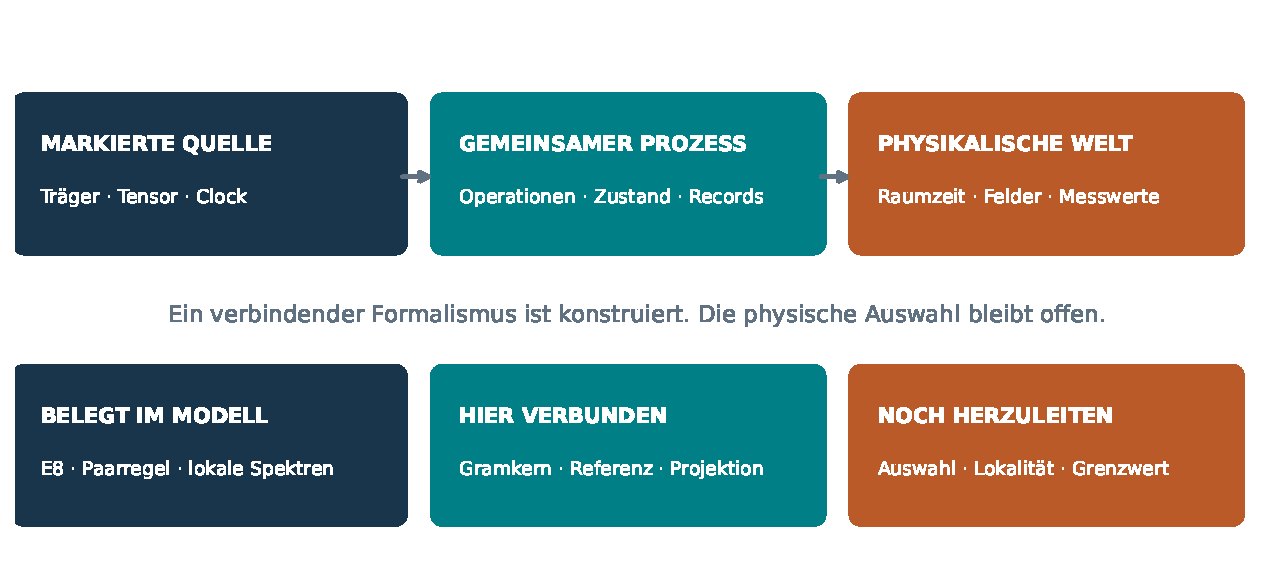
\includegraphics[keepaspectratio,alt={Die gemeinsame Kette und ihre Beweisgrenzen. Die drei unteren Felder unterscheiden vorliegende Modellresultate, eigene Verbindungen und die noch fehlende physische Ableitung.}]{figures/01_gemeinsame_kette.pdf}}
\caption{Die gemeinsame Kette und ihre Beweisgrenzen. Die drei unteren
Felder unterscheiden vorliegende Modellresultate, eigene Verbindungen
und die noch fehlende physische Ableitung.}
\end{figure}

\section{1. Fragestellung, Quellenstand und wissenschaftliche
Reichweite}\label{fragestellung-quellenstand-und-wissenschaftliche-reichweite}

\subsection{1.1 Was „ganzheitlich`` hier
bedeutet}\label{was-ganzheitlich-hier-bedeutet}

Eine ganzheitliche Theorie benötigt mehr als Ergebnisse mit ähnlichen
Dimensionszahlen. Sie muss zeigen, dass ihre Algebra, ihr Zustand, ihre
Dynamik und ihre Messungen zusammenpassen. Wenn ein Grundzustand in
Modell A, ein Transport in Modell B und ein chirales Feld in Modell C
berechnet werden, entsteht daraus erst dann eine gemeinsame Physik, wenn
explizite Abbildungen die jeweiligen Annahmen und beobachtbaren Prozesse
miteinander verbinden.

Daher lautet die Leitfrage dieses Papers:

Welche einheitlichen Ausgangsdaten bestimmen
\((\mathcal A,\alpha_t,\omega,\mathfrak I)\) und deren physikalische
Interpretation?

Hier ist \(\mathcal A\) eine Algebra von Observablen, \(\alpha_t\) ihre
Entwicklung, \(\omega\) ein Zustandsfunktional und \(\mathfrak I\) die
Familie tatsächlich zugelassener Instrumente. Ein Instrument umfasst die
möglichen Messausgänge samt Zustandsänderung und Wahrscheinlichkeit. Die
Notation ist eine Spezifikation; sie wählt diese Daten noch nicht aus.

Anschaulich beschreibt die bisherige TFPT-Grammatik, welche Bauteile
zusammenpassen. Eine vollständige Ausführung muss zusätzlich erklären,
welche Handgriffe vorkommen, was anfänglich vorliegt und welche Spuren
die Handgriffe hinterlassen. Raum wäre dann eine besondere Struktur
unabhängiger Zugriffsmöglichkeiten und endlicher Signalwege. Zeit wäre
mehr als die Ordnung einer zyklischen Matrix: Sie müsste als gemeinsame
Entwicklung mit lesbaren Korrelationen auftreten.

\subsection{1.2 Quellenhierarchie und
Stichtag}\label{quellenhierarchie-und-stichtag}

Der Ausgangskorpus umfasst 74 eingefrorene Dokumentdateien
einschließlich des nachgereichten Texts. Darunter befinden sich elf PDFs
mit zusammen 830 Seiten; ihre Texte wurden extrahiert. Die zentralen und
neu geänderten Abschnitte wurden gezielt gelesen, repräsentative
Ausgangsseiten visuell kontrolliert. Die Zahl der inventarisierten
Seiten bedeutet ausdrücklich keinen vollständigen erneuten Beweisaudit
jeder historischen Aussage.

Die Hauptquellen sind:

\begin{itemize}
\tightlist
\item
  \textbf{S046:} Hauptdokument v1.6 vom 15. September, 168 PDF-Seiten;
  breite historische und physikalische Grundlage.
\item
  \textbf{S033:} Clock/Gemeinsame-Quelle-Konsolidierung v1.6.6; innere
  Spin-Identifikation, Operationsverträge, Transferzeuge und
  Feldkorrekturen.
\item
  \textbf{S001:} andere v1.6.6-Linie, „Fundamentale Fortsetzung``;
  Präparationslücke, quantitative Restantwort, Trennschnitte und
  Feldstabilität.
\item
  \textbf{S003:} fundamentale Reduktion; symmetrische Gesamtantwort,
  Multiplizitätsräume und operationaler Wirkungstest.
\item
  \textbf{S068/S070:} Ergebnisbericht und vollständige Konsolidierung
  v1.6.7; korrekte H-Kette, Singulettprojektionen, bilineare Zerlegung
  und Unterbestimmtheit.
\item
  \textbf{S074:} jüngster Nachtrag derselben v1.6.7 mit nativer
  Kodierung, Schattenrekonstruktion, Interventionsgegenbeispiel und
  Z4-/Bogoliubov-Analyse.
\item
  \textbf{S071/S072:} zentrale offene Probleme und Compiler-Synthese des
  Repositorys.
\end{itemize}

S001 und S033 sind verschiedene Dokumentlinien trotz gleicher
Versionsnummer. Inhalt, Tensorpin und Beweisvoraussetzungen entscheiden
über ihre Kombination. S070 bewahrt große Teile älterer Fassungen als
historische Anhänge; das bloße Wiederauftauchen einer Aussage ist kein
neuer Beweis. In der vorliegenden Synthese stehen jeweils die neuesten
kompatiblen Aussagen im Haupttext.

Das Repository hatte bei der Bestandsaufnahme den Commit
\texttt{66b91e40e245} (vollständiger Hash im Prüfpaket), aber viele
neuere, nicht eingecheckte Forschungsdateien. Deshalb bezeichnet der
Commit allein den hier ausgewerteten Stand nicht. Das Quellenmanifest
hält die tatsächlich verwendeten Dateien mit SHA-256 fest. Aktive fremde
Forschungsarbeiten wurden nicht verändert. Die Hauptsynthese
berücksichtigt auch den während der Arbeit hinzugekommenen Nachtrag
S074. Die früher eingefrorenen Fassungen bleiben zum Versionsvergleich
erhalten; der letzte inhaltliche Nachtrag wurde am 15.09.2026 gegen
12:30 Uhr MESZ gesichert.

\subsection{1.3 Beweisstatus}\label{beweisstatus}

\textbf{Gesetzt} sind Modellannahmen und Ressourcenzugänge.
\textbf{Exakt} ist eine Identität oder ein mathematischer Schluss unter
genannten Voraussetzungen. \textbf{Numerisch} bezeichnet eine
Approximation ohne rigoroses Intervall. \textbf{Bedingt} bedeutet, dass
ein Resultat zusätzliche, noch nicht hergeleitete Eingaben benötigt.
\textbf{Offen} kennzeichnet fehlende Beweise oder physikalische
Identifikationen.

„Exakt`` und „bedingt`` können zugleich gelten. Beispielsweise ist die
Ladungserhaltung der neuen Referenzkonstruktion exakt; dass TFPT diese
Referenz erzeugt, bleibt offen. Ein bewiesener Satz über ein
festgelegtes Modell ist außerdem noch keine empirische Bestätigung
dieses Modells.

Die eigenen Rechnungen umfassen 57 explizite exakte Prüfbedingungen,
darunter native Tensoridentitäten, eine vollständige
Graphcharakteristik, rationale Ritz-Einschließung, symbolische
Referenzkopplung und Projektorgeometrie. Normaler und optimierter Lauf
stimmen bytegenau überein. Zusätzlich wurde der 20 Bedingungen
umfassende H-Ketten-Prüfer aus v1.6.7 in einer isolierten Kopie
ausgeführt. Der große historische Grundzustandslauf und die vollständige
Vier-Boson-Enumeration wurden hier nicht erneut gerechnet. Ihre
Voraussetzungen bleiben entsprechend sichtbar.

\section{2. Die algebraische Grundlage: was TFPT tatsächlich
zusammenbindet}\label{die-algebraische-grundlage-was-tfpt-tatsuxe4chlich-zusammenbindet}

\subsection{2.1 Ausgangsstruktur und
Einheiten}\label{ausgangsstruktur-und-einheiten}

Die historische Kurzfassung organisiert sich um

\[c_3=\frac1{8\pi},\qquad g_{\mathrm{car}}=5.\]

Der zweite Ausdruck ist eine Trägerzahl, nicht die Kopplung \(g\) des
späteren Hamiltonoperators. Die erste Eingabe enthält mehr als eine
Zahl: orientierte Rand- oder Nahtstruktur, einen geeigneten positiven
Kern und eine Normierung. Die zweite benötigt einen konkreten komplexen
Träger und Markierungen. Diese Daten dürfen nicht verschwinden, wenn man
die Theorie verbal auf „zwei Zahlen`` verkürzt. {[}S046, Kap. 3; S072,
§2{]}

Der fünfteilige Träger liefert

\[S^+=\Lambda^{\mathrm{even}}\mathbb C^5,
\qquad \dim S^+=1+10+5=16.\]

Das ist die chirale Spinordarstellung der inneren Gruppe
\(\mathrm{Spin}(10)\). Daraus folgt noch nicht, dass die physikalische
Raumzeit zehn- oder fünfdimensional wäre. Ebenso ist der arithmetische
Familienzähler \((16-1)/5=3\) kein Beweis dreier leichter chiraler
Familien.

Eine dimensionslose Theorie kann Verhältnisse vorhersagen. Die Angabe
einer Energie in GeV benötigt zusätzlich einen Bezug zu einer
dimensional kalibrierten Größe. Einheitenwahl und Vorhersage
dimensionsloser Verhältnisse sind getrennte Fragen; die Verwendung einer
eingesetzten Planckskala muss im physikalischen Anschluss dokumentiert
bleiben.

\subsection{\texorpdfstring{2.2 Von \(D_5\oplus A_3\) zu
\(E_8\)}{2.2 Von D\_5\textbackslash oplus A\_3 zu E\_8}}\label{von-d_5oplus-a_3-zu-e_8}

Beide Wurzelgitter haben Determinante vier. Eine geeignete diagonale
Verklebung ihrer Diskriminantklassen erzeugt einen geraden Überverband
vom Index vier. Seine Determinante ist

\[\det L=\frac{\det D_5\det A_3}{4^2}=1.\]

Mit Positivität und Rang acht erhält man das gerade unimodulare
\(E_8\)-Gitter. Die Aussage benötigt die Verklebungsform; die Rangsumme
\(5+3=8\) allein reicht nicht. Die 240 Wurzeln sind 112 ganzzahlige
Wurzeln mit zwei Einträgen \(\pm1\) und 128 Halbvektoren mit gerader
Minusparität. {[}S046, Kap. 3{]}

Die komplexe Lie-Algebra zerfällt als

\[
\mathfrak e_8=(45,1)\oplus(1,15)\oplus(16,4)
\oplus(\overline{16},\overline4)\oplus(10,6).
\]

Die Dimensionen summieren sich zu 248. Insbesondere treten dieselben 64
und 60 auf, die später den nativen Paarvertrag tragen. Diese
Übereinstimmung ist strukturell relevant, weil ein konkreter Intertwiner
die Paarung realisiert. Sie ersetzt dennoch keine Auswahl von Energie,
Zustand oder räumlicher Ausführung.

\subsection{2.3 Der kleine Matrixkern}\label{der-kleine-matrixkern}

Im gemeinsamen Matrixkörper \(M_2(\mathbb Q(i))\) seien

\[
a=iI_2,\quad
u_1=\begin{pmatrix}i&0\\0&-i\end{pmatrix},\quad
u_2=\begin{pmatrix}0&1\\-1&0\end{pmatrix},\quad
u_3=u_1u_2,
\]

Die Familie wird durch

\[w=\frac12(I+u_1+u_2+u_3),\qquad w^3=-I\]

ergänzt. Mit \(D=\mathbb Z[i]\) und

\[P=\begin{pmatrix}1&(1+i)^{-1}\\0&(1+i)^{-1}\end{pmatrix}\]

liegt eine maximale Ordnung \(\mathcal M=PM_2(D)P^{-1}\) vor. Unter der
reellen Form

\[\langle A,B\rangle=\operatorname{Re}\operatorname{Tr}(AB^\dagger)\]

hat ihre ganzzahlige Acht-Basis positive führende Hauptminoren
\(2,4,4,4,4,4,2,1\). Die Form ist gerade und unimodular: wiederum
\(E_8\). Die Quellen enthalten außerdem eine markierungstreue Abbildung
zum tatsächlich verwendeten Compiler-Gitter. {[}S046, Kap. 34{]}

Das ist stärker als eine zufällige Zahlengleichheit. Gleichwohl sind nur
96 der 240 Wurzelmatrizen unitär; 144 haben Rang eins. Eine Wurzel ist
somit nicht automatisch eine ausführbare reversible Zeitoperation.
Verschiedene Ordnungen können dieselbe hermitesche Kegelansicht haben
und sich in ihren nicht-hermiteschen Operationen unterscheiden. Der
positive Kegel wählt den vollständigen Operationssatz nicht allein aus.

\subsection{2.4 Der Clock-Anschluss}\label{der-clock-anschluss}

Die neuere native Clock-Konstruktion verwendet eine Permutation auf fünf
Hilfsachsen und ihre vorzeichenrichtige Exteriorhebung. Mit zehn
Majorana-Matrizen \(\gamma_j\), der Parität \(\Pi\) und

\[R_{ab}=\tfrac12(\gamma_a-\gamma_b)(\gamma_{a+5}-\gamma_{b+5})\]

wird explizit

\[S=\gamma_0\cdots\gamma_9R_{01}R_{02}R_{34}
=\Pi\Gamma(p)\in\mathrm{Spin}(10).\]

Die Wirkung auf gerade Spinoren und Vektoren reproduziert die beiden
nativen Darstellungen und erhält den Tensor. Dieser Clock hat Ordnung
sechs. {[}S033, §3{]}

Frühere Ordnung-3-Familienoperationen und Ordnung-12-Lifts gehören zu
ihren jeweils bezeichneten Darstellungen. Matrixordnung, projektive
Ordnung und Ordnung der Konjugationswirkung sind getrennt zu prüfen.
Ihre Zahlen werden hier nicht zu einer einzigen universellen
Periodizität zusammengezogen. Der neue Satz verbindet einen konkreten
Clock mit der inneren Symmetrie; er liefert weder kontinuierliche
Symmetriekontrollen noch eine Zeiteinheit.

\section{3. Universalraum als Prozess: Zustand, Gedächtnis und
Schatten}\label{universalraum-als-prozess-zustand-geduxe4chtnis-und-schatten}

\subsection{3.1 Das endliche
Kontextmodell}\label{das-endliche-kontextmodell}

Im markierten komplexen Viererträger liegen 60 Strahlen in 15
orthogonalen Viererkontexten vor. Bei der festgelegten Inzidenzregel
\(B\) und gleichmäßiger Wahl der sieben zulässigen Nachfolgekontexte
gilt

\[
T_{(D,t),(C,s)}=\frac{B_{DC}}7
\operatorname{Tr}(\Pi_{D,t}\Pi_{C,s}).
\]

Jeder Ausgang besitzt einen Übergang mit Gewicht \(1/7\) und zwölf mit
Gewicht \(1/14\). Die genaue Faktorisierung führt zu Rang 30 und dem
Spektrum

\[\{1^{[1]},(2/7)^{[9]},(-2/7)^{[5]},(3/7)^{[15]},0^{[30]}\}.\]

Die Born-Regel, die zulässigen Kontexte und deren Gewichtung sind dabei
Eingaben. Der stationäre Systemzustand \(I_4/4\) ist ein Fixpunkt dieses
Messprozesses; er ist nicht bereits das physikalische Vakuum. {[}S046,
Kap. 4{]}

\subsection{3.2 Warum eine einzige Dichtematrix nicht immer
genügt}\label{warum-eine-einzige-dichtematrix-nicht-immer-genuxfcgt}

Für klassische Kontextinformation und ein Quantensystem kann man einen
Zustand durch positive Blöcke \(X_C\) beschreiben. Die feste Ausführung
lautet

\[\Phi(X)_D=\sum_C K_{DC}\Delta_D(X_C).\]

Die Quellen zeigen \(\operatorname{rank}\Phi=60\) und
\(\operatorname{rank}\Phi^2=30\). Für eine bestimmte passive
Marginalauslesung schließen sogar 45 lineare Größen. Dagegen können
selektive Eingriffe oder wiederverwendete kohärente Register mehr
Information zugänglich machen. Die minimale Beschreibung hängt somit vom
tatsächlichen Operations- und Auslesevertrag ab. {[}S046, Kap. 5{]}

Ein System kann nach einer Vormessung dieselbe reduzierte Dichtematrix
haben, obwohl sein gemeinsamer Zustand mit einem behaltenen Register
eine andere spätere Antwort liefert als mit einem frischen Register. Das
ist kein Widerspruch: Die gemeinsame Korrelation fehlt in der
reduzierten Beschreibung. Die etablierte Theorie von Quantennetzwerken
und Prozesstensoren beschreibt genau solche Mehrzeitverträge. {[}E1,
E2{]}

\subsection{3.3 Aufzeichnungen müssen die richtige Interferenz
erhalten}\label{aufzeichnungen-muxfcssen-die-richtige-interferenz-erhalten}

Für den antisymmetrischen Paaradapter

\[K:\mathbb C^4\otimes\mathbb C^4\longrightarrow\Lambda^2\mathbb C^4\]

gilt in der hier verwendeten Normierung

\[K^\dagger K=I-\mathsf S,\]

mit dem Swap \(\mathsf S\). Die Wege \(ab\) und \(ba\) treffen denselben
Vermittler mit entgegengesetztem Vorzeichen. Fügt man orthogonale
Records an diese zwei Wege an, verschwinden ihre Kreuzterme. Man erhält
stattdessen \(I-D_{\mathrm{diag}}\), wobei
\(D_{\mathrm{diag}}=\sum_a|aa\rangle\langle aa|\).

Damit verändert eine unpassende Aufzeichnung die Dynamik. Kanten dürfen
als verschiedene Ereignisse unterscheidbar bleiben; vertauschte innere
Wege derselben antisymmetrischen Paarung müssen kohärent bleiben. Die
Aussage ist nicht „History ist unmöglich``, sondern eine konkrete
Verträglichkeitsbedingung an ihre Gramstruktur. {[}S072, Nachtrag N3{]}

Allgemein gilt für zwei lineare Adapter desselben Eingangsraums:

\[L^\dagger L=K^\dagger K
\quad\Longleftrightarrow\quad L=VK\]

mit einer Isometrie \(V\) auf \(\operatorname{ran}K\). Der Beweis steht
in Abschnitt 8. Diese einfache Identität wird zum ersten Bestandteil
einer gemeinsamen Rekonstruktion.

\section{4. Die Vierträgerzelle und die Grenze lokaler
Modelllösungen}\label{die-viertruxe4gerzelle-und-die-grenze-lokaler-modellluxf6sungen}

Der total antisymmetrische Zustand

\[|\Omega_4\rangle=\frac1{\sqrt{24}}
\sum_{\pi\in S_4}\operatorname{sgn}(\pi)
|\pi(0)\pi(1)\pi(2)\pi(3)\rangle\]

ist ein \(SU(4)\)-Singulett. Seine Einteilchenreduktionen sind
\(I_4/4\), seine Paarreduktionen \((I-\mathsf S_{ij})/12\). Die Ordnung
liegt in den Beziehungen, obwohl jedes einzelne Teil maximal gemischt
aussieht.

Für

\[H_{\mathrm{tet}}=J\sum_{i<j}P^+_{ij},\qquad
P^+_{ij}=\tfrac12(I+\mathsf S_{ij}),\quad J>0\]

ist \(\Omega_4\) der eindeutige Nullzustand. Fordert man dieselbe
vollständige Antisymmetrie bei mehr als vier Viererträgern, ist
\(\Lambda^n\mathbb C^4=0\) für \(n>4\). Eine globale Welt kann deshalb
nicht aus beliebig vielen gleichzeitig perfekt erfüllten solchen
Paarbedingungen entstehen. Frustration, andere Verklebung oder andere
Freiheitsgrade werden wesentlich. {[}S046, Kap. 6--8{]}

Für zwei vollständige Tetramer mit der festgelegten positiven
Einzelbrücke existiert ein allkoppliger Grundzustandssatz. Mit
\(\lambda\ge0\) und

\[R=\sqrt{16J^2-2J\lambda+\lambda^2},\qquad
Q=\sqrt{4J^2+\lambda^2}\]

gilt

\[E_0=\tfrac12(4J+\lambda-R),\qquad
\operatorname{gap}=J+\tfrac12(R-Q)>J/2.\]

Historische Schwellen \(\lambda=8J\) waren Grenzen schwächerer Beweise,
keine Phasenübergänge dieses Modells. Dieser Satz betrifft zwei Zellen
und die bezeichnete Brücke. Er ist weder eine uniforme Vielzellenaussage
noch der Grundzustandssatz der nativen 64/60-Bank.

Ein Produkt eindimensionaler Singulettgrundräume ist selbst
eindimensional. Projiziert man vollständig darauf, bleibt nur eine
skalare Energie. Nichttriviale niedrige Dynamik benötigt Anregungen,
Randfreiheiten oder Multiplizitäten. Diese Beobachtung verbindet das
Zellmodell mit der späteren Frage, wo Raum überhaupt mathematisch Platz
haben kann.

\section{5. Die native Bank: festgelegte Dynamik und gesicherte
Antwort}\label{die-native-bank-festgelegte-dynamik-und-gesicherte-antwort}

\subsection{5.1 Modellvertrag und
Tensor}\label{modellvertrag-und-tensor}

Die native Konstruktion verwendet Fermionoperatoren \(f_i\) für
\(i=1,\dots,64\), Bosonoperatoren \(b_A\) für \(A=1,\dots,60\) und

\[
P_A=\sum_{i<j}W_{A,ij}f_jf_i,\qquad
H_{\mathrm{nat}}=\Delta N_b+g\sum_A(b_A^\dagger P_A+P_A^\dagger b_A).
\]

Es gelten \(\Delta>0\), reelles \(g\) und

\[N=N_f+2N_b,\qquad [H_{\mathrm{nat}},N]=0.\]

\(W\) hat 480 Einträge \(\pm1\), acht disjunkte Paare je Zeile und
\(WW^\dagger=8I_{60}\). Die Fermionen tragen \((16,4)\), die Bosonen
\((10,6)\) unter der inneren Gruppe. Der verwendete Tensorpin lautet:

\texttt{3f00a0892157a691e4ef26920c3702772c7bf76a250fad98ff04a079bb64b763}.

Der Tensor und seine Gramidentität wurden in dieser Arbeit frisch
geprüft. Die gesamte Fockbank ist wegen der Bosonen
unendlichdimensional; jeder feste nichtnegative \(N\)-Sektor ist
endlichdimensional. „Endliche Bank`` bedeutet daher eine endliche Zahl
von Moden, nicht automatisch einen endlichen Gesamthilbertraum.

\subsection{5.2 Grundzustand und
Entnahmelinie}\label{grundzustand-und-entnahmelinie}

Der übernommene native Satz gilt für den \(\mu=0\)-Vertrag und
\(0<|g|/\Delta\le1/20\): Der globale Grundzustand ist eindeutig und
liegt bei \(N=64\). Am Betriebspunkt \(g/\Delta=1/20\) geben die
bisherigen Zertifikate

\[-1.158089<E_0/\Delta<-1.129636,
\qquad 0.842846<\langle N_b\rangle<1.245656.\]

Die neue v1.6.7-Kompression verschärft die Obergrenze zu

\[\boxed{-1.158089<E_0/\Delta<-1.12963811.}\]

Für die isolierte niedrige Entnahmelinie im \(N=63\)-Sektor gilt damit

\[\boxed{0.00773911<\epsilon/\Delta<0.039079764,}\]

sowie das übernommene Gewicht

\[Z_{\mathrm{low}}>\frac{40912436089}{46487375000}>0.88007628.\]

Die Normierung ist wesentlich: \(Z_{\mathrm{low}}\) bezieht sich auf das
gesamte normierte Fermionspektralgewicht je Mode. Die gesamte
Entnahmenorm ist dagegen
\(\nu=\langle f_r^\dagger f_r\rangle=1-\langle N_b\rangle/32\). Ein
isolierter Pol im endlichen Sektor ist zunächst eine isolierte
Eigenlinie; seine Identifikation als relativistisches Teilchen verlangt
Dispersion, Feldadapter und Grenzwert. {[}S033, §1; S068, §4{]}

\subsection{5.3 Weshalb eine schwächere Sonde den stärkeren Satz nicht
widerlegt}\label{weshalb-eine-schwuxe4chere-sonde-den-stuxe4rkeren-satz-nicht-widerlegt}

Ein paralleler Arbeitsstand konnte den Grundzustand mit seinen eigenen
gröberen Schranken bei \(g/\Delta=1/20\) nicht isolieren. Er verlangte
dazu Energieobergrenzen, die mit dem stärkeren früheren Intervall
unvereinbar wären. Daraus folgt, dass diese Sonde zu schwach ist. Es
folgt weder eine neue niedrigere Energie noch die Widerlegung des
vorhandenen nativen Satzes. Ebenso ist ein Ritzwert oberhalb einer
bekannten besseren Obergrenze keine neue Grundenergie.

Versionskonflikte betreffen auch Prüfberichte: In einer früheren Datei
war eine Nichtschlussnorm um \(229^2\) falsch skaliert. Die aktuellen
Korrekturen verwenden

\[\|w_2\|^2=\frac{5001523200}{229}>0.\]

Solche Unterschiede werden durch Dateipins und direkte Rechnung
entschieden, nicht durch das Wort PASS im Bericht. {[}S033, §2; S068,
§2{]}

\subsection{5.4 Zustandswahl ist eine zusätzliche physikalische
Frage}\label{zustandswahl-ist-eine-zusuxe4tzliche-physikalische-frage}

Die Familie

\[H_\mu=H_{\mathrm{nat}}+\mu N\]

bewahrt dieselbe innere Symmetrie. Für neutrale \(O\) mit \([O,N]=0\)
gilt bei demselben Anfangszustand exakt

\[e^{itH_\mu}Oe^{-itH_\mu}=e^{itH_{\mathrm{nat}}}Oe^{-itH_{\mathrm{nat}}}.\]

Dennoch verändert \(\mu\) den Vergleich verschiedener Ladungssektoren.
Die dokumentierte Schranke bei \(\mu=\Delta/50\) und \(g=\Delta/20\)
wählt das leere Vakuum. Symmetrie und neutrale Daten allein bestimmen
somit den globalen Zustandsvertrag nicht. In einem festgehaltenen
Gesamtsektor ist \(\mu N\) dagegen nur eine Konstante und kein
beobachtbarer Unterschied. Eine fundamentale Theorie benötigt Auswahl
nur bis auf Gleichheit aller zugelassenen Prozesse. {[}S046, Kap. 36;
S003, §6{]}

\subsection{5.5 Der native Tensor als verlustfreier
Kodierer}\label{der-native-tensor-als-verlustfreier-kodierer}

Der während der Synthese hinzugekommene Nachtrag zu v1.6.7 macht eine
weitere Verbindung explizit. Aus derselben Gramidentität folgt

\[V=\frac{W^\dagger}{\sqrt8}:\mathbb C^{60}\longrightarrow\Lambda^2\mathbb C^{64},
\qquad V^\dagger V=I_{60},\qquad
\Pi=VV^\dagger=\frac{W^\dagger W}{8}.\]

Ein logischer Zustand mit 60 Komponenten hat damit eine verlustfreie
Darstellung als kohärenter Fermionpaarzustand. Die Rückabbildung sieht
jedoch nur einen Rang-60-Teilraum der insgesamt 2016 Paarrichtungen; ihr
Kern ist 1956-dimensional. Diese dunklen Richtungen sind für diese
Abbildung unsichtbar, nicht allgemein bedeutungslos. Im hellen
\(N=2\)-Bereich lautet die gemeinsame Dynamik exakt

\[H_{2,\mathrm{hell}}=
\begin{pmatrix}0&\sqrt8g\\\sqrt8g&\Delta\end{pmatrix}\otimes I_{60}.\]

Sie wandelt Paar- und Bosondarstellung ineinander um. Bei
\(g/\Delta=1/20\) beträgt die maximale Umwandlungswahrscheinlichkeit
\(2/27\). Der allein in die Paarseite eingebettete Code ist für
\(g\ne0\) kein invarianter Hamiltonunterraum. Dies ist eine konkrete
Verbindung zweier Ansichten desselben \(N=2\)-Prozesses; sie
identifiziert diesen Prozess nicht mit dem Grundzustand in \(N=64\).
{[}S074, B5.1{]}

\textbf{Ein präziser Schutztest.} Für jede einzelne Fermionmode ergibt
sich

\[\operatorname{spec}(V^\dagger n_rV)
=\{0\text{ mit Vielfachheit }45,\quad
\tfrac18\text{ mit Vielfachheit }15\}.\]

Die Besetzung ist auf dem logischen Raum nicht skalar. Eine verlorene
Mode kann daher Information über den kodierten Zustand an die Umgebung
geben. Der gesamte 60-dimensionale Code korrigiert die beliebige
Löschung einer einzelnen Mode nicht. Die Kompressionen aller 64 Moden
wurden für dieses Paper am eingefrorenen Tensor erneut exakt geprüft.
Kleinere Untercodes und kontrolliert zusammengesetzte Kodierungsnetze
bleiben mögliche Forschungsrichtungen. Isometrie allein begründet weder
Fehlerkorrektur noch eine holografische Raumgrenze. Etablierte
holografische Codes liefern dafür zusätzliche Rekonstruktions- und
Schutzbedingungen. {[}S074, B5.2; E11; E12{]}

\subsection{5.6 Die Z4-Erweiterung: erlaubte Dynamik und echte neue
Parameter}\label{die-z4-erweiterung-erlaubte-dynamik-und-echte-neue-parameter}

Der neueste Nachtrag zeigt außerdem, dass die Erhaltung von \(N\)
stärker ist als die innere Symmetrie allein verlangt. Ein auf jedem Grad
konstanter ganzzahliger Lift der betrachteten Z4-Klammern müsste

\[2q_1=q_2,\qquad q_1+q_3=0,\qquad2q_3=q_2\]

erfüllen. Die Koeffizientenmatrix besitzt Determinante vier; ganzzahlig
bleibt nur der triviale Lift. Das widerlegt keine anderen Cartanladungen
und setzt die E8-Lieklammer nicht mit primitiven CAR-Operatoren gleich.
{[}S074, B4{]}

Die reelle symmetrische invariante Bosonpaarung \(\eta\) mit
\(\eta^2=I\) erlaubt am selben Tensor zusätzlich

\[B_+=\frac12b^\dagger\eta b^\dagger,\qquad
R_+=b^\dagger\eta P^\dagger.\]

Beide Operatoren sind \(G\)-invariant, ändern \(N\) um vier und erhalten
\(N\bmod4\). Innerhalb der ausdrücklich begrenzten Klasse
normalgeordneter, fermionparitätsgerader, \(G\)-invarianter Polynome vom
Grad höchstens drei ergibt sich

\[\begin{aligned}
H_{\mathrm{ext}}={}&c+\varepsilon N_f+\Delta N_b
+\kappa B_++\overline\kappa B_-\\
&+g\sum_A b_A^\dagger P_A
+\overline g\sum_A P_A^\dagger b_A
+\lambda R_++\overline\lambda R_-.
\end{aligned}\]

Die Quellenprüfung der vollen Generatoren zeigt die Zulässigkeit. Sie
leitet die Kopplungen nicht aus dem Ursprung ab. Die nativen
Grundzustands- und Polschranken gelten für diese Erweiterung nicht
automatisch. \(N\bmod4\) ist außerdem bereits durch das Zentrum von
\(SU(4)\) realisiert. Der Übergang von neun auf acht kontinuierliche
diagonale Phasenerhaltungen bedeutet nicht, dass die volle innere Gruppe
verschwände. Ein zusätzlicher \(\mu N\)-Term bleibt \(G\)- und
Z4-invariant; die Auswahlfrage bleibt bestehen. Für \(\Delta>|\kappa|\)
lässt sich die Energie nach unten beschränken, doch daraus folgt noch
kein eindeutiger neuer Grundzustand. {[}S074, B4.1{]}

\textbf{Wann ist die Erweiterung nur eine andere Beschreibung?} In der
reellen, phasengleichen Familie führt die kanonische Transformation

\[b=c\cosh r+\eta c^\dagger\sinh r\]

zu

\[\begin{aligned}
\Delta'&=\Delta\cosh2r+\kappa\sinh2r,&
\kappa'&=\Delta\sinh2r+\kappa\cosh2r,\\
g'&=g\cosh r+\lambda\sinh r,&
\lambda'&=g\sinh r+\lambda\cosh r.
\end{aligned}\]

Für \(g^2>\lambda^2\) lassen sich die beiden zusätzlichen Terme durch
diese uniforme Transformation gleichzeitig entfernen genau dann, wenn

\[\boxed{\mathcal I=\kappa(g^2+\lambda^2)-2\Delta g\lambda=0.}\]

Die additive Konstante ist \(30(\Delta'-\Delta)\). Bei
\(\mathcal I\ne0\) ist diese spezielle Reduktion ausgeschlossen; ein
Satz über alle denkbaren verborgenen Symmetrien folgt nicht. Die
einfache Familie \(\lambda=g\), \(\kappa=0\) entgeht einer solchen
endlichen Reduktion und ist ein konkreter Kandidat für weitere
Forschung. Bei \(\varepsilon=0\) besitzen beide kubischen Kanäle
dieselbe freie Frequenz \(\Delta\); ein bloßes Argument mit schneller
und langsamer Rotation erklärt ihr unterschiedliches Behalten nicht.
{[}S074, B4.2{]}

Dieser Nachtrag verbessert die fundamentale Fragestellung erheblich:
Zuerst müssen physikalisch verschiedene Dynamiken von bloßen
Variablenwechseln getrennt werden. Erst danach kann eine Ursprungsregel
sinnvoll auswählen. Die Auswahl erfolgt also auf Klassen gleicher
vollständiger Prozesse, was unmittelbar an Abschnitt 8 anschließt.

\section{6. Der neueste Stand v1.6.7: die richtige kleine
Rechenkette}\label{der-neueste-stand-v1.6.7-die-richtige-kleine-rechenkette}

\subsection{6.1 Vier Singuletts auf der zweiten
Bosonstufe}\label{vier-singuletts-auf-der-zweiten-bosonstufe}

Sei \(F\) der vollständig gefüllte Fermionzustand ohne Bosonen. Bei
\(k\) Bosonen gibt es im \(N=64\)-Sektor \(2k\) Löcher. Der invariante
Teil liegt in

\[\mathcal S_k=
[\Lambda^{2k}(\overline{16\otimes4})\otimes
\operatorname{Sym}^k(10\otimes6)]^G.\]

Die ersten Dimensionen sind \(1,1,4\). Die vierte Richtung bedeutet
keinen vierten Grundzustand, sondern einen größeren Raum möglicher
Singulettkombinationen.

Auf der Bosonseite gilt

\[\operatorname{Sym}^2(10\otimes6)=
(1,1)\oplus(54,1)\oplus(1,20')\oplus(54,20')\oplus(45,15).\]

Der skalare \((1,1)\)-Typ hat keinen passenden Beitrag in der
betreffenden Fermionstufe. Die vier übrigen gemeinsamen Typen liefern
die vollständige Singulettbasis. Für \(v_2=T_+^2F\) lauten die
Normquadrate und Kopplungen:

{\def\LTcaptype{none} % do not increment counter
\begin{longtable}[]{@{}lrr@{}}
\toprule\noalign{}
Typ & \(\|P_Rv_2\|^2\) & quadrierte Kopplung/\(g^2\) \\
\midrule\noalign{}
\endhead
\bottomrule\noalign{}
\endlastfoot
\((54,1)\) & 17280 & 36 \\
\((1,20')\) & 7680 & 16 \\
\((54,20')\) & 241920 & 504 \\
\((45,15)\) & 172800 & 360 \\
Summe & 439680 & 916 \\
\end{longtable}
}

Die vollständige Kompression bis einschließlich dieser Stufe ist

\[
P_{\le2}HP_{\le2}\simeq
\begin{pmatrix}
0&g\sqrt{480}&0\\
g\sqrt{480}&\Delta&g\sqrt{916}\\
0&g\sqrt{916}&2\Delta
\end{pmatrix}\oplus2\Delta I_3.
\]

Sie ist exakt bestimmt, aber nicht invariant: Übergänge zur nächsten
Bosonstufe bleiben. Ihre Eigenwerte sind Variationsdaten, nicht
automatisch Eigenwerte des vollständigen Operators. {[}S068, §3{]}

\subsection{6.2 Lanczos zählt Hamiltonschritte, nicht
Bosonen}\label{lanczos-zuxe4hlt-hamiltonschritte-nicht-bosonen}

Die einfache Kette entsteht aus \(F,HF,H^2F,\ldots\) durch
Orthogonalisierung:

\[Hu_n=b_nu_{n-1}+a_nu_n+b_{n+1}u_{n+1}.\]

Die aktuellen Koeffizienten sind

\[\frac{(a_0,a_1,a_2,a_3,a_4)}\Delta
=\left(0,1,2,3,\frac{105168998}{26292551}\right),\]

\[\frac{(b_1^2,b_2^2,b_3^2,b_4^2)}{g^2}
=\left(480,916,\frac{299520}{229},\frac{78877653}{47632}\right).\]

Der fünfte Vektor enthält sowohl \(v_4\) als auch \(w_2\). Er hat keine
feste Bosonzahl. Eine Kettenlänge von höchstens 33 folgt deshalb nicht
aus den 33 möglichen Bosonzahlen. Der Lanczosindex ist ein Rechenindex;
seine Deutung als räumlicher Ort wäre ein zusätzlicher unbegründeter
Schritt.

Die fünf Glieder bestimmen die zehn Momente
\(\mu_n=\langle F,H^nF\rangle\) für \(0\le n\le9\). Ein Weg zum
ausgelassenen sechsten Kettenvektor und zurück braucht mindestens zehn
Schritte. Insbesondere

\[\mu_2=480g^2,\quad \mu_3=480\Delta g^2,\quad
\mu_4=480\Delta^2g^2+670080g^4.\]

Diese Momente gehören \(F\), nicht \(\Omega\) und nicht den geladenen
Antwortoperatoren. Die rationale Sturm-Einschließung der kleinsten
Ritzenergie

\[-1.12963813<E_{\mathrm{Ritz},5}/\Delta<-1.12963811\]

wurde hier unabhängig aus den gegebenen Koeffizienten nachvollzogen. Der
Ursprung des übernommenen vierten Bosonmoments wurde nicht neu
enumeriert. {[}S068, §4{]}

\subsection{6.3 Ein exakter Nachweis fehlender
Auswahl}\label{ein-exakter-nachweis-fehlender-auswahl}

Aus den Momenten folgt

\[\frac{\mu_4\mu_2}{\mu_3^2}=1+1396(g/\Delta)^2.\]

Das ergibt \(4.49\) bei \(g/\Delta=1/20\), aber \(1.8725\) bei \(1/40\).
Beide Modelle besitzen dasselbe \(W\), dieselben inneren Symmetrien und
denselben kommutierenden Clock. Die dimensionslose Differenz ist keine
Einheitenfrage. Damit ist belegt, dass diese Grunddaten allein die
physikalische Dynamik nicht eindeutig auswählen. Die Referenz \(F\) muss
für eine tatsächliche Messung verfügbar sein; die algebraische
Ungleichheit der Prozesse ist davon getrennt. {[}S068, §8{]}

\subsection{6.4 Nachgereichter Text: die interessante Fortsetzung liegt
in
Matrixmomenten}\label{nachgereichter-text-die-interessante-fortsetzung-liegt-in-matrixmomenten}

Der während dieser Arbeit nachgereichte Text \emph{Operationssatz,
nativer Grundzustand und Feldwörterbuch}, beschriftet als v1.6.3, ist
byteidentisch mit dem bereits gelesenen aktuellen Repositorybericht
derselben Linie. Sein Tensor, Lochbild, Kommutantenstufen und
Nichtschlussbefund sind deshalb bereits berücksichtigt. Seine Priorität
„den Zwei-Boson-Singulettraum ausschreiben`` ist in v1.6.7 inzwischen
durch die vier expliziten Richtungen erfüllt. Die pauschale Behauptung,
der nichtskalare Clock liege außerhalb der zusammenhängenden Gruppe, ist
durch das konkrete Spin-Wort überholt. {[}S073; S033, §3; S068, §3{]}

\textbf{Eine weiterhin interessante Richtung steckt in seinen
Onishi-/Wick-Spurnetzwerken.} Sie berechnen hohe Bosonstufennormen, ohne
sämtliche Fockamplituden auszuschreiben. Der Nichtschluss beweist
jedoch, dass die skalaren Normen \(\nu_k\) allein nicht genügen. Die
natürliche Weiterentwicklung sind gemischte Wortmomente und
projektoraufgelöste Matrixmomente, beispielsweise

\[\Gamma_{(R,u),(R',v)}
=\langle uP_Rv_2,vP_{R'}v_2\rangle.\]

Hier sind \(u,v\) ausdrücklich Wörter in \(H\), \(T_+\), \(T_-\) und den
benötigten tatsächlichen Observablen. Solche Matrizen behalten
Kreuzterme zwischen den vier Richtungen und nachfolgenden Bosonstufen.
Sie passen genau zum Prozesskern aus Abschnitt 8. Ein tensorbasierter
Kontraktionsalgorithmus dafür könnte die gemeinsame Rechnung wesentlich
verkleinern, ohne den verzweigten Raum irrtümlich zu einer einzigen
Bosonleiter zu machen. Die Entwicklung und Ausführung dieses erweiterten
Kontraktionsalgorithmus ist in diesem Paper nicht bereits erfolgt.

Eine dazu passende \textbf{exakte analytische Fortsetzung} ist die
Blockresolvente. Für eine orthogonale Zerlegung und

\[H=\begin{pmatrix}A&B^\dagger\\B&D\end{pmatrix}\]

gilt für \(\operatorname{Im}z\ne0\)

\[P(z-H)^{-1}P
=\big[z-A-B^\dagger(z-D)^{-1}B\big]^{-1}.\]

Dies folgt durch Eliminieren der zweiten Blockzeile. Der Rest
verschwindet nicht; er erscheint als energieabhängige Selbstenergie. Für
\(\eta=|\operatorname{Im}z|>0\) und endliche selbstadjungierte Blöcke
folgt

\[\|\Sigma(z)\|\le\|B\|^2/\eta,\qquad
\|P(z-H)^{-1}P-(z-A)^{-1}\|\le\|B\|^2/\eta^3.\]

Die erste Schranke benutzt \(\|(z-D)^{-1}\|\le1/\eta\), die zweite die
Resolventenidentität und die Schranken \(1/\eta\) für beide äußeren
Resolventen. Diese Kontrolle wird nahe der reellen Achse schwach;
präzise Polaussagen benötigen eine bessere Rest- und Abstandskontrolle.
Sie ist trotzdem ein klarer Erfolgstest für die vorgeschlagene
Spurnetzwerkfortsetzung: nicht nur weitere Normen berechnen, sondern die
tatsächliche Matrixrestkopplung der gemeinsamen Antwort einschließen.

Die Feldgradierungen des Textes bleiben ebenfalls als Kandidaten
relevant. Die dort genannten Aufteilungen 24/36 oder 40/20 sind
ansatzgebundene Vektor-/Tensorkanäle, keine Auswahl eines gesunden
relativistischen Parents. Der nächste Gewinn wäre ein vollständiger
positiver Feldvertrag für genau einen solchen Ansatz mit nachgewiesener
Rückführung auf W. Die Aussage „einziger einheitlicher Feldtyp`` gilt
nur in der abgegrenzten Ein-Kopie-, Händigkeit- und Ableitungsklasse.

\section{7. Präparation, Restantwort und die Herkunft von
Teilen}\label{pruxe4paration-restantwort-und-die-herkunft-von-teilen}

\subsection{7.1 Ein kontrollierter Weg in den nativen
Grundzustand}\label{ein-kontrollierter-weg-in-den-nativen-grundzustand}

Die zweite v1.6.6-Linie betrachtet

\[H(s)=\Delta N_b+sgX,\quad0\le s\le1\]

im festen \(N=64\)-Sektor. Der Startzustand \(F\) ist dort bei \(s=0\)
eindeutig. Aus einer Komplementuntergrenze und Variationsobergrenzen
folgt eine durchgehende Lücke

\[\operatorname{gap}H(s)>
\frac{97697}{1187646}\Delta>0.0822610441\Delta.\]

Mit einer konservativen quantitativen Adiabatenschranke erhält man bei
\(T\Delta=10^9\) einen Fehlerbetrag unter \(0.000523\) und eine
Grundzustandswahrscheinlichkeit über \(99.9999726\%\). Das ist ein
mathematisch bedingter Präparationssatz unter steuerbarer Rampe und
verfügbarem \(F\), keine durchgeführte Rampensimulation oder
Laborpräparation. Die globale Nullenergieentartung bei \(s=0\) stört
diesen festen Sektor nicht, solange die Ladung exakt erhalten bleibt.
{[}S001, §2; Adiabatensatz E3{]}

\subsection{7.2 Die volle Antwort ist nicht exakt
zweilinienförmig}\label{die-volle-antwort-ist-nicht-exakt-zweilinienfuxf6rmig}

Mit \(b=\langle N_b\rangle\) und

\[S=15-\frac7{32}b,\quad a=\frac{\Delta b-E_0}{64}\]

lauten die bisherigen normierten Spektralmomente

\[m_0=1,\quad m_1=0,\quad m_2=g^2S,\quad
m_3=g^2(\Delta S+7a).\]

Für den zweiten orthogonalen Operatorrest folgt

\[\rho^2=m_4-\frac{m_3^2}{m_2}-m_2^2,\qquad
\beta_2^2=\rho^2/m_2.\]

Die neue Restidentität liefert unter den nativen Voraussetzungen

\[\operatorname{Var}(N_b)>0.1193989,
\qquad\beta_2^2>9.640875\cdot10^{-7}\Delta^2.\]

Der Koeffizient ist eine Kopplung an den restlichen Antwortbereich. Er
ist weder dessen prozentuales Gewicht noch eine punktweise Schranke der
vollständigen Selbstenergie. Eine brauchbare Näherung benötigt außerdem
eine obere Fehlerkontrolle im gewünschten Frequenzfenster. {[}S001,
§3{]}

\subsection{7.3 Eine Bank ist in ihrer ursprünglichen Modenbasis stark
verbunden}\label{eine-bank-ist-in-ihrer-urspruxfcnglichen-modenbasis-stark-verbunden}

Die frische Rechnung am gepinnten \(W\) ergibt 480 Kanten auf 64
Fermionmoden, Grad 15 und das exakte Adjazenzspektrum

\[15^{[1]},\quad3^{[25]},\quad(-1)^{[30]},\quad(-5)^{[3]},\quad(-9)^{[5]}.\]

Die Laplacelücke ist zwölf. Für eine Teilmenge mit \(s\) Moden gilt
deshalb

\[|\partial S|\ge \frac{12s(64-s)}{64}
=\frac{3s(64-s)}{16}.\]

Ein 32/32-Schnitt kreuzt mindestens 192 Paarterme. Der Beweis nutzt den
zentrierten Indikator \(1_S-(s/64)\mathbf1\): Sein Laplacequadratikwert
zählt die Schnittkanten und seine Norm ist \(s(64-s)/64\).

Das erklärt, weshalb das bloße Aufteilen der ursprünglichen Koordinaten
keine zwei unabhängigen Banken ergibt. Es beweist keine Raumdimension
und schließt anders konstruierte emergente Lokalität nicht aus. Eine
neue lokale Basis müsste Operatoren, Zustand und Auslesung gemeinsam
transformieren. {[}S001, §4; eigene Tensorprüfung{]}

\section{8. Eigene Verbindung I: ein gemeinsamer
Prozesskern}\label{eigene-verbindung-i-ein-gemeinsamer-prozesskern}

\subsection{8.1 Die zentrale
Vereinfachung}\label{die-zentrale-vereinfachung}

Die bisherigen Teilprobleme können auf ein gemeinsames mathematisches
Objekt bezogen werden: die Überlappungen aller tatsächlich zulässigen
Operationsgeschichten. Sei \(\mathcal W\) die Menge endlicher Wörter aus
einem ausdrücklich festgelegten Alphabet von Operationen und ihren
Adjungierten. Auf einem gemeinsamen Startzustand \(\Omega\) definiere

\[\boxed{\Gamma(u,v)=\langle u\Omega,v\Omega\rangle
=\omega(u^\dagger v).}\]

Dieser \textbf{Prozesskern} umfasst nicht allein Wahrscheinlichkeiten
einzelner Ausgänge. Seine komplexen Kreuzterme halten fest, welche
Geschichten noch interferieren können. Werden Register und Apparate in
den gemeinsamen Raum aufgenommen, gehören auch ihre Zustandsänderungen
zu den Wörtern.

Die Idee ist mathematisch mit der GNS-Rekonstruktion positiver
Funktionale verwandt. Für gemischte Anfangszustände kann man entweder
das Funktional direkt verwenden oder eine gemeinsame Reinigung mitsamt
unzugänglicher Umgebung führen. Die hier ausgeschriebene Anwendung ist
ein Verbindungssatz für die TFPT-Arbeitsstände, kein literaturweiter
Neuheitsanspruch.

\subsection{8.2 Satz: Rekonstruktion aus einem vollständigen positiven
Wortkern}\label{satz-rekonstruktion-aus-einem-vollstuxe4ndigen-positiven-wortkern}

\textbf{Voraussetzungen.} Gegeben seien eine unital abgeschlossene
\(*\)-Algebra \(\mathfrak A\) der zulässigen Wörter, ihre Relationen und
ein normiertes positives Funktional \(\omega\) mit \(\omega(1)=1\). Für
eine Darstellung durch beschränkte Operationen werde zusätzlich für
jeden Generator \(a\) eine Schranke

\[\omega(x^\dagger a^\dagger ax)\le C_a^2\omega(x^\dagger x)
\qquad(x\in\mathfrak A)\]

verlangt. In endlichdimensionalen konkreten Modellen ist diese Bedingung
erfüllt. Ein unbeschränkter Hamiltonoperator benötigt außerhalb dieser
Fassung eigene Definitionsbereichs- und Selbstadjungiertheitskontrolle.

\textbf{Aussage.} Es gibt einen Hilbertraum \(\mathcal H_\omega\), einen
zyklischen Vektor \(\Omega_\omega\) und eine Darstellung \(\pi\) mit

\[\omega(a)=\langle\Omega_\omega,\pi(a)\Omega_\omega\rangle.\]

Auf dem von allen Wörtern erzeugten Raum ist diese Darstellung bis auf
unitäre Äquivalenz eindeutig.

\textbf{Beweis.} Auf \(\mathfrak A\) setze man
\(\langle x,y\rangle=\omega(x^\dagger y)\) und quotiente die
Nullvektoren aus. Positivität liefert Cauchy--Schwarz. Die
Generatorenschranke zeigt, dass ein Nullvektor nach Linksanwendung von
\(a\) wieder ein Nullvektor ist. Also ist \(\pi(a)[x]=[ax]\)
wohldefiniert und beschränkt. Die Vervollständigung ergibt den
Hilbertraum; \([1]\) ist zyklisch. Zwei solche Realisierungen haben auf
allen endlichen Linearkombinationen derselben Wörter dieselben
Skalarprodukte. Die Zuordnung \(u\Omega\mapsto u\widetilde\Omega\) ist
daher wohldefiniert und isometrisch und erweitert sich wegen Zyklizität
zu einer unitären Abbildung. \(\square\)

Der Satz erklärt, in welchem Sinn ein „Universalraum`` als gemeinsamer
erreichbarer Prozessraum präzise sein kann. Er setzt jedoch den
vollständigen positiven Kern und das Operationsalphabet voraus. Eine
einzelne endliche Momentenmatrix genügt weder für eine eindeutige
unendliche Fortsetzung noch für physikalische Lokalität.

Für ein physikalisches Instrument müssen zusätzlich die
Ausgangsoperatoren \(M_j\) eine vollständige Operation bilden, etwa
\(\sum_jM_j^\dagger M_j=I\) für einen spurtreuen Gesamtprozess. Die
Wahrscheinlichkeiten sind dann \(\omega(M_j^\dagger M_j)\); selektive
Zweige behalten ihre tatsächliche Ausbeute. Positivität allein setzt
diese Normierungs- und Kompositionsrelationen nicht ein.

\textbf{Mehrere Schatten derselben Quelle.} Bei festgelegten linearen
Reduktionen \(R_i\) ist eine endliche uneingeschränkte Zustandsklasse
genau dann gemeinsam unterscheidbar, wenn auf hermiteschen spurlosen
Differenzen \(\bigcap_i\ker R_i=\{0\}\) gilt. Alle echten Teilmarginalen
von \((|000\rangle\pm|111\rangle)/\sqrt2\) sind dagegen gleich; erst
eine phasensensitive gemeinsame Messung wie \(XXX\) unterscheidet sie.
Auch passende paarweise Überschneidungen garantieren noch keine
gemeinsame globale Realisierung. Das Wortkernkriterium verlangt daher
gemeinsame zulässige Operationen einschließlich der relevanten
Kreuzterme. Es rekonstruiert den zyklisch erreichbaren Raum, keinen
völlig entkoppelten dunklen Zusatzsektor. {[}S074, B5.3{]}

\subsection{8.3 Zustandswahl und Dynamik lassen sich nicht durch
Rekonstruktion
erschleichen}\label{zustandswahl-und-dynamik-lassen-sich-nicht-durch-rekonstruktion-erschleichen}

Der Satz konstruiert aus vorhandenen Prozessdaten eine gemeinsame
Darstellung. Er erzeugt diese Daten nicht aus E8 allein. Die Familie
\(H_{\Delta,g}\) aus Abschnitt 6 zeigt ausdrücklich, dass gleiche
Grammatik verschiedene positive Prozesskerne zulässt. Ebenso können
verschiedene Anfangszustände auf derselben Algebra verschiedene
Funktionale liefern.

Für eine kontinuierliche Zeitentwicklung benötigt man zusätzlich eine
konsistente, ausreichend stetige Automorphismengruppe \(\alpha_t\). In
einer invariant gewählten GNS-Darstellung kann sie unter den üblichen
Voraussetzungen unitär implementiert werden. Eine einparametrige Gruppe
und ihre Stetigkeit fallen nicht aus einer Ordnung-6-Clock heraus. Der
Energie-Nullpunkt und die positive Energiebedingung müssen ebenfalls
korrekt behandelt werden.

Der wissenschaftliche Gewinn liegt deshalb in einer scharfen Reduktion:
Die gemeinsame Herkunft wird zur Auswahl eines \textbf{positiven,
zeitlich konsistenten, lokal komponierbaren Prozesskerns}. Das ist ein
präziseres Ziel als eine Liste voneinander unabhängiger schöner
Matrizen.

\subsection{8.4 Kompatibilitätssatz für verschiedene
Arbeitsstände}\label{kompatibilituxe4tssatz-fuxfcr-verschiedene-arbeitsstuxe4nde}

Angenommen, zwei Konstruktionen verwenden dasselbe Wortalphabet und
besitzen für \textbf{alle} zulässigen Wörter denselben Gramkern. Dann
sind ihre zyklischen Ausführungen unitär äquivalent und die
entsprechende Unitäre verschränkt sämtliche Generatoren. Gleichheit nur
von \(\Gamma(1,u)\) oder wenigen Wahrscheinlichkeiten genügt nicht.

Der lokale Recordsatz ist der einfachste Spezialfall. Ist
\(K^\dagger K=L^\dagger L\), definiert man \(V(Kx)=Lx\). Aus \(Kx=0\)
folgt \(\|Lx\|^2=0\), also ist die Definition wohldefiniert. Sie erhält
Skalarprodukte und ist auf dem Bild isometrisch. Umgekehrt ergibt
\(L=VK\) unmittelbar die Gramgleichheit.

Für ganze Prozesse lautet die entsprechende Prüffrage:

\[\langle u\Omega,v\Omega\rangle
\stackrel{?}=\langle\widetilde u\widetilde\Omega,
\widetilde v\widetilde\Omega\rangle\]

für dieselben Eingriffe, Referenzen und Ausgänge. Damit wird verhindert,
dass ein N=9-Transferzeuge, eine N=4-Zellreferenz und die
N=64-Grundzustandsantwort ohne Adapter als eine einzige Lösung gelten.

\subsection{8.5 Ein endlicher Fehlervertrag für
Adapter}\label{ein-endlicher-fehlervertrag-fuxfcr-adapter}

Sei \(J:\mathcal H_{\mathrm{eff}}\to\mathcal H\) eine Isometrie,
\(h=J^\dagger HJ\) und

\[R=HJ-Jh=(I-JJ^\dagger)HJ.\]

Für endliche selbstadjungierte Matrizen gilt durch die Duhamel-Identität

\[\boxed{\|e^{-itH}J-Je^{-ith}\|\le |t|\,\|R\|.}\]

\textbf{Beweis.} Man differenziert \(e^{-i(t-s)H}Je^{-ish}\) nach \(s\),
integriert von null bis \(t\) und benutzt die Norm eins beider unitären
Faktoren. Für negatives \(t\) folgt dieselbe Schranke mit \(|t|\).
\(\square\)

Bei einem Effekt \(0\le E\le I\) ist der Unterschied der
Ausgangswahrscheinlichkeiten zweier so verglichener normierter Zustände
höchstens \(2|t|\|R\|\). Damit erhält das Wort „gemeinsam`` einen
zahlenmäßigen Inhalt: Eine behauptete effektive Wirkung muss größer als
die kontrollierte Adapterunsicherheit sein. Bei langen Zeiten kann die
lineare Schranke unbrauchbar werden; dann benötigt man bessere spektrale
oder lokale Abschätzungen. Die Methode ersetzt insbesondere keine
uniforme Kontrolle im thermodynamischen Limes.

\section{9. Eigene Verbindung II: Transfer mit mitgerechneter
Ladungsreferenz}\label{eigene-verbindung-ii-transfer-mit-mitgerechneter-ladungsreferenz}

\subsection{9.1 Was der vorhandene Vierzustandszeuge bereits
leistet}\label{was-der-vorhandene-vierzustandszeuge-bereits-leistet}

Im wirklichen Tensor \(W\) existieren die Paarungen \((4,57)\) in Kanal
0 und \((4,58)\) in Kanal 1. Mit den sieben Pauli-Blockern

\[S_b=\{8,16,28,32,44,52,56\}\]

und einem zusätzlich gewährten Bosonmischer schließt die vollständige
Paarwechselwirkung auf den vier N=9-Zuständen

\[
|1\rangle=S_b+\{4,57\},\quad |2\rangle=S_b+b_0,
\quad |3\rangle=S_b+b_1,\quad |4\rangle=S_b+\{4,58\}.
\]

Nach Phasenwahl ist der exakte Block

\[H_4=\begin{pmatrix}
0&g&0&0\\g&\Delta&J&0\\0&J&\Delta&g\\0&0&g&0
\end{pmatrix}.\]

Die Quellen beweisen seine Invarianz unter sämtlichen nativen
Paartermen; es handelt sich nicht um eine willkürliche
Vierzustandsabschneidung. Für

\[g/\Delta=1/20,\quad J/\Delta=1-1/(10\sqrt3),
\quad t\Delta=20\pi\sqrt3\]

gilt

\[P_{1\to4}>\frac{2009992727}{2022609600}>0.99376208.\]

Der Mischer verändert allerdings eine erhaltene innere Cartanladung mit
Werten \((7,7,9,9)\). Er ist aus dem bisherigen diese Ladung erhaltenden
Alphabet nicht erzeugbar. Die native Teilchenladung \(N=9\) ist eine
andere Größe und bleibt schon im ursprünglichen Block erhalten. {[}S033,
§5{]}

\subsection{9.2 Explizite ladungserhaltende
Erweiterung}\label{explizite-ladungserhaltende-erweiterung}

\textbf{Neue Konstruktion, bedingt.} Ergänze eine zweidimensionale
Referenz mit Zuständen \(|+\rangle,|-\rangle\) und

\[Q_R|\pm\rangle=\pm|\pm\rangle,\qquad
R_-=|-\rangle\langle+|.\]

Schreibe \(Q_S=\operatorname{diag}(7,7,9,9)\) und
\(M=|3\rangle\langle2|\). Dann gilt

\[[Q_S,M]=2M,\qquad [Q_R,R_-]=-2R_-.\]

Für \(H_0=H_4|_{J=0}\) definiere

\[
\boxed{H_{\mathrm{rel}}=H_0\otimes I
+J(M\otimes R_-+M^\dagger\otimes R_-^\dagger)
+\kappa I\otimes Q_R^2.}
\]

Dieser achtdimensionale Hamiltonoperator ist selbstadjungiert und
erfüllt exakt

\[[H_{\mathrm{rel}},Q_S\otimes I+I\otimes Q_R]=0.\]

Der Raum

\[\mathcal K=\operatorname{span}\{
|1,+\rangle,|2,+\rangle,|3,-\rangle,|4,-\rangle\}\]

hat durchgehend Gesamtladung acht. Er ist invariant, und in dieser Basis
gilt

\[H_{\mathrm{rel}}|_{\mathcal K}=H_4+\kappa I_4.\]

\textbf{Beweis.} Die beiden nativen Endkopplungen ändern \(Q_S\) nicht.
Der mittlere Übergang erhöht \(Q_S\) um zwei und erniedrigt gleichzeitig
\(Q_R\) um zwei. Keine der drei Kopplungen verlässt die vier angegebenen
Zustände. Wegen \(Q_R^2=I\) ist der Referenzenergieterm dort skalar. Die
Einschränkung ist daher genau die behauptete Matrix. Alle Identitäten
wurden symbolisch geprüft. \(\square\)

Damit wird die vorhandene Transferwahrscheinlichkeit unverändert auf die
erweiterte Konstruktion übertragen. Der Endzustand ist nun
\(|4,-\rangle\) statt \(|4,+\rangle\). Die mitgerechnete Referenz
erklärt exakt, wohin die fehlende Cartanladung geht.

\begin{figure}
\centering
\pandocbounded{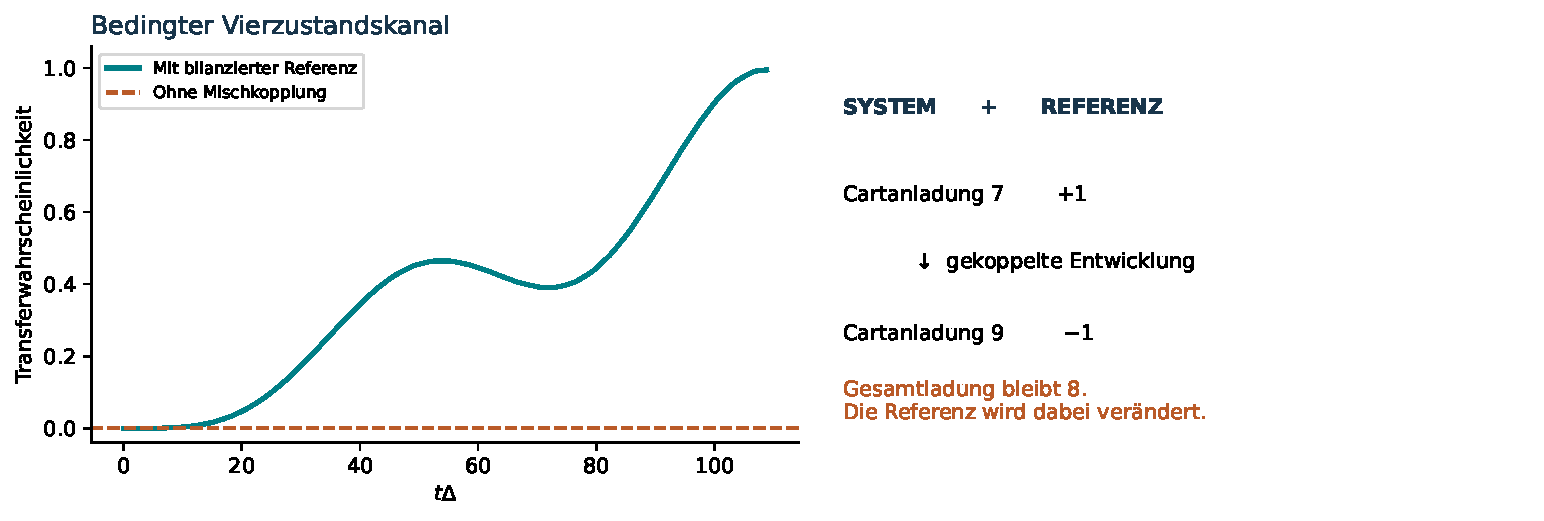
\includegraphics[keepaspectratio,alt={Bedingter relationaler Transfer. Links: numerische Zeitkurve des exakt definierten Vierzustandsblocks; die rigorose Endpunktschranke stammt aus S033. Rechts: die neue exakte Ladungsbilanz. Die Referenz und ihre gekoppelte Operation sind zusätzliche Ressourcen.}]{figures/02_relationaler_transfer.pdf}}
\caption{Bedingter relationaler Transfer. Links: numerische Zeitkurve
des exakt definierten Vierzustandsblocks; die rigorose Endpunktschranke
stammt aus S033. Rechts: die neue exakte Ladungsbilanz. Die Referenz und
ihre gekoppelte Operation sind zusätzliche Ressourcen.}
\end{figure}

\subsection{9.3 Was damit fundamental gelöst wird -- und was
nicht}\label{was-damit-fundamental-geluxf6st-wird-und-was-nicht}

Gelöst ist die konkrete mathematische Frage, ob die festgestellte
Cartan-Schranke einen Transfer auch bei mitgeführtem Ladungsausgleich
grundsätzlich verbietet. Das tut sie nicht: Die Erweiterung liefert
einen expliziten positiven Zeugen. Sie bewahrt die betrachtete
Gesamt-Cartanladung, ohne den ursprünglichen isolierten Mischer als
bereits verfügbar auszugeben.

Die Konstruktion leitet weder die Referenzzustände noch die gekoppelte
Operation aus TFPT ab. Sie behauptet auch keine Erhaltung der
vollständigen inneren Gruppe durch diese Erweiterung. Dafür müssten
vollständige Darstellungen, alle anderen Ladungen und passende
Intertwiner ergänzt und geprüft werden. Die Referenz wurde lediglich für
die einzelne konkret blockierende Cartanladung gebaut. Ihr
physikalischer Träger und ihre sonstigen Quantenzahlen sind offene
Eingaben.

Allgemein kann eine Operation \(M_q\) mit \([Q_S,M_q]=qM_q\) durch eine
Referenzoperation \(R_{-q}\) mit \([Q_R,R_{-q}]=-qR_{-q}\) zu einem
neutralen Produkt ergänzt werden. Dieses Prinzip ist in der Theorie von
Quantenreferenzen und Superselektion bekannt. Hier wird es auf den
vorhandenen nativen Transferblock angewandt und vollständig
ausgerechnet. {[}E4{]}

\subsection{9.4 Die Referenz wird verbraucht: ein einfacher
Unmöglichkeitssatz}\label{die-referenz-wird-verbraucht-ein-einfacher-unmuxf6glichkeitssatz}

Beginnt die Referenz in einer scharfen Ladung \(r\) und erhöht sich die
Systemladung in einem erfolgreichen Zweig um \(q\ne0\), muss die
Referenz oder eine weitere Umgebung im selben Zweig ihre Ladung um
\(-q\) ändern. Ein vollständiger Rücklauf zur exakt gleichen scharfen
Referenzladung bei sonst unverändertem Außenraum ist wegen
Gesamtladungserhaltung unmöglich.

Für die obige Konstruktion sind \(|+\rangle\) und \(|-\rangle\)
orthogonal. Eine zweistufige Referenz ist für einen solchen scharfen
einmaligen Ausgleich minimal; ein eindimensionaler Träger kann keinen
nichtverschwindenden Ladungswechsel aufnehmen. Eine unveränderte
Wiederverwendung verlangt Rücktransport, ein weiteres Reservoir oder
einen anderen Referenzvertrag. Dies ist keine kostenlose katalytische
Operation.

Damit werden Zustandspräparation, Aufzeichnung und Transport miteinander
verbunden: Der Ausgang enthält eine reale Änderung einer mitgerechneten
Ressource. Bei Superpositionen kann sie zudem welche-Zweig-Information
tragen. Wer sie wegtraziert, muss den Verlust von Systemkohärenz in die
Prozessrechnung aufnehmen.

\section{10. Eigene Verbindung III: Überlappung, Dynamik und
geometrische
Krümmung}\label{eigene-verbindung-iii-uxfcberlappung-dynamik-und-geometrische-kruxfcmmung}

\subsection{10.1 Eine gemeinsame Quelle ist nicht automatisch
Bewegung}\label{eine-gemeinsame-quelle-ist-nicht-automatisch-bewegung}

Sei \(T:\mathbb C^m\to\mathcal H\) ein Adapter, dessen Spalten die
betrachteten Zustände sind. Dann

\[S=T^\dagger T,\qquad K=T^\dagger HT.\]

Ist \(S>0\), erhält man mit \(J=TS^{-1/2}\) einen isometrischen Adapter
und

\[h=J^\dagger HJ=S^{-1/2}KS^{-1/2}.\]

Bei singulärem \(S\) wird zuerst sein Nullraum entfernt. Ist
\(K=\epsilon S\), dann ist \(h=\epsilon I\). Offdiagonale Einträge in
\(K\) können also vollständig durch die nichtorthogonale Beschriftung
entstehen. Für tatsächliche Dynamik muss zusätzlich die Kopplung zum
ausgelassenen Raum kontrolliert werden; Abschnitt 8.5 liefert dafür
einen einfachen Vertrag.

Auf dem einzelnen entarteten nativen Lochpol gilt genau
\(P_hHP_h=E_hP_h\). Neue Charts innerhalb dieses Polraums ergeben
zwangsläufig \(K=E_hS\). Sie erzeugen durch bloße Überlappung keine
räumliche Ausbreitung. Die neue gemeinsame Quelle muss wirklich mehr als
eine neue Benennung dieser Zustände liefern. {[}S033, §7{]}

\subsection{10.2 Zeitabhängige Rahmen brauchen einen
Verbindungsterm}\label{zeitabhuxe4ngige-rahmen-brauchen-einen-verbindungsterm}

Für einen glatten isometrischen Rahmen \(J(t)\) und \(\psi(t)=J(t)c(t)\)
ergibt die projizierte Schrödingergleichung

\[\boxed{i\dot c=(J^\dagger HJ-iJ^\dagger\dot J)c.}\]

Der zweite Term ist nötig, weil die Koordinaten selbst bewegt werden.
Eine Rechnung, die nur \(J^\dagger HJ\) betrachtet, kann eine
Rahmendrehung fälschlich als physische Dynamik lesen. Bei einem echten
bewegten Unterraum muss die außerhalb liegende Gleichung ebenfalls
erfüllt oder durch eine adiabatische beziehungsweise andere
Fehlerabschätzung kontrolliert werden.

Wählt man \(J(t)=J_0V(t)\) innerhalb eines festen Unterraums, ist die
zusätzliche Struktur reine Rahmenwahl. Eine Vorhersage für einen
festgelegten Detektor darf davon nicht abhängen. Deshalb müssen
Zustände, Generator und Messinstrument zusammen transformiert werden.

\subsection{10.3 Feste vollständige Rahmen und bewegte Projektoren
unterscheiden
sich}\label{feste-vollstuxe4ndige-rahmen-und-bewegte-projektoren-unterscheiden-sich}

Sind \(U_{xy}=V_x^\dagger V_y\) bloße Basiswechsel vollständiger
unitärer Rahmen, teleskopiert eine geschlossene Schleife:

\[U_{xy}U_{yz}U_{zx}=I.\]

Anders ist es für isometrische Einbettungen \(J_x\) echter Unterräume
mit \(P_x=J_xJ_x^\dagger\). Dann

\[J_x^\dagger J_yJ_y^\dagger J_zJ_z^\dagger J_x
=J_x^\dagger P_yP_zJ_x,\]

und dies muss nicht die Identität sein. Die Zwischenprojektionen sind
zusätzliche geometrische beziehungsweise physische Struktur. Die
Überlappungsmatrizen sind im Allgemeinen keine unitären
Transportoperatoren; ihre Beträge und mögliche
Erfolgswahrscheinlichkeiten müssen erhalten bleiben.

Mit der hermiteschen Verbindung \(A=iJ^\dagger dJ\) ist die Krümmung

\[\boxed{F=dA-iA\wedge A
=i\,dJ^\dagger(I-P)\wedge dJ.}\]

\textbf{Herleitung.} Aus \(J^\dagger J=I\) folgt
\(dJ^\dagger J=-J^\dagger dJ\). Einsetzen in \(dA-iA\wedge A\) trennt
den vollen Ausdruck in den Anteil innerhalb und außerhalb von \(P\); der
innere Anteil hebt sich weg. Ist \(P\) konstant und ändern sich nur
seine Rahmen, verschwindet \(F\). Bewegt sich der physische Unterraum,
kann \(F\ne0\) sein. \(\square\)

Das ist die etablierte Berry-/Wilczek--Zee-Struktur, hier als konkrete
Antwort auf das Überlappungsproblem eingesetzt. Sie ist noch kein
dynamisches Yang--Mills-Feld der Raumzeit. {[}E5{]}

\subsection{10.4 Ein vollständig gerechneter kleiner
Zeuge}\label{ein-vollstuxe4ndig-gerechneter-kleiner-zeuge}

Betrachte die normierte Familie

\[u(\theta,\phi)=
\begin{pmatrix}\cos(\theta/2)\\e^{i\phi}\sin(\theta/2)\end{pmatrix},
\qquad P=uu^\dagger.\]

Direkte Rechnung ergibt

\[A_\theta=0,\quad A_\phi=-\sin^2(\theta/2),
\quad F_{\theta\phi}=-\tfrac12\sin\theta.\]

Aus demselben Projektor folgt die reelle Quantenmetrik

\[ds^2=\operatorname{Re}\langle du,(I-P)du\rangle
=\tfrac14(d\theta^2+\sin^2\theta\,d\phi^2).\]

\textbf{Der verbindende Punkt:} Unterscheidbarkeit und geometrische
Phase stammen hier aus demselben komplexen Tangentialprodukt. Die Metrik
ist sein reeller Teil, die Krümmung hängt an seinem antisymmetrischen
imaginären Teil. Es müssen also nicht zwei unabhängige Strukturen frei
eingesetzt werden. Die Parametrisierung des Projektors selbst bleibt
aber eine Eingabe.

\begin{figure}
\centering
\pandocbounded{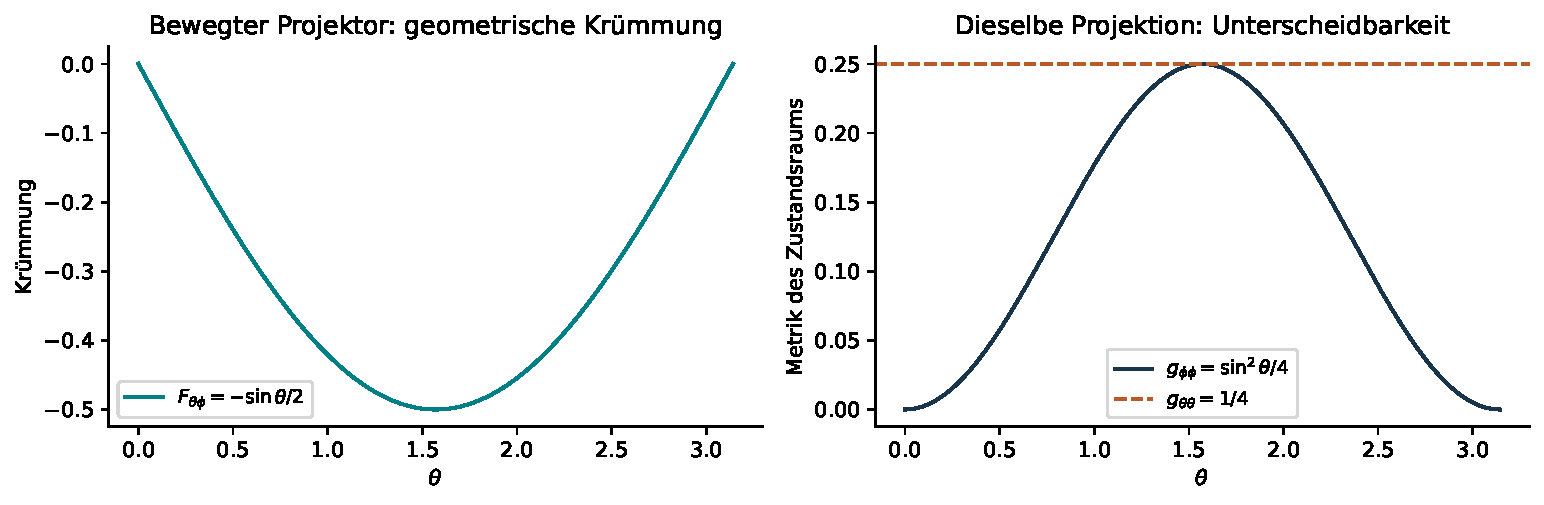
\includegraphics[keepaspectratio,alt={Derselbe bewegte Rang-eins-Projektor liefert geometrische Krümmung und Zustandsmetrik. Die Achsen sind Modellparameter; sie sind keine bereits abgeleiteten Raumzeitkoordinaten.}]{figures/03_projektorgeometrie.pdf}}
\caption{Derselbe bewegte Rang-eins-Projektor liefert geometrische
Krümmung und Zustandsmetrik. Die Achsen sind Modellparameter; sie sind
keine bereits abgeleiteten Raumzeitkoordinaten.}
\end{figure}

Eine endliche Kontrolle verwendet

\[u_0=(1,0)^T,\quad u_1=(1,1)^T/\sqrt2,
\quad u_2=(1,i)^T/\sqrt2.\]

Das rahmeninvariante Dreiecksprodukt ist

\[\langle u_0,u_1\rangle\langle u_1,u_2\rangle
\langle u_2,u_0\rangle=(1+i)/4.\]

Seine Phase ist \(\pi/4\), sein Normquadrat \(1/8\). Die selektive
Projektionsfolge \(P_1\), dann \(P_2\), dann \(P_0\) auf \(u_0\) hat
entsprechend Wahrscheinlichkeit \(1/8\) und Amplitude \((1-i)/4\). Die
umgekehrte Orientierung erklärt das Vorzeichen der Phase. Ein Normieren
jedes Schritts ohne seine Ausbeute würde diese reale Ressourcenzahl
unterschlagen. Alle angegebenen Identitäten wurden symbolisch geprüft.

\subsection{10.5 Ein bedingter dynamischer
Parent}\label{ein-bedingter-dynamischer-parent}

Der zusätzliche Hamiltonoperator

\[H(\theta,\phi)=\Delta(I-P(\theta,\phi))\]

hat bei festem Parameter eine Lücke \(\Delta\) und einen
Rang-eins-Grundraum \(P\). Bei kontrollierter langsamer
Parameteränderung liefert er die bekannte geometrische Phase, mit
separat zu kontrollierendem adiabatischem Fehler. Er zeigt konstruktiv,
dass ein bewegter ausgewählter Unterraum die falsche „alles
teleskopiert``-Abkürzung umgehen kann.

Er leitet weder die Parameter noch ihre Raumzeitinterpretation aus TFPT
ab. Ein elementarer geometrischer Phasenraum ist auch kein masseloser
Eichboson. Dafür müssten \(P_x\) oder entsprechende Verbindungsdaten
selbst dynamisch werden, aus einer Quelle stammen und eine positive
lokale Wirkung samt geeignetem Grenzverhalten besitzen.

Das ist ein aussichtsreicher \textbf{bedingter Verbindungsansatz}:
Anstelle willkürlich hinzugefügter Eichpotentiale könnte man die
Geometrie quellseitig ausgewählter niedriger Unterräume untersuchen. Der
unmittelbar entscheidende Test lautet, ob der native Operationssatz
einen physisch veränderlichen Projektor erzeugt. Bewegt er nur den
Rahmen eines festen \(P\), ist dieser Kandidat beendet.

\section{11. Wo Raum und echte Wirkung entstehen
könnten}\label{wo-raum-und-echte-wirkung-entstehen-kuxf6nnten}

\subsection{11.1 Innere Darstellung und
Multiplizität}\label{innere-darstellung-und-multiplizituxe4t}

Unter einer kompakten inneren Gruppe zerfällt ein endlicher Hilbertraum
als

\[\mathcal H=\bigoplus_\lambda R_\lambda\otimes\mathcal M_\lambda.\]

Ein gruppeninvarianter Hamiltonoperator hat die Form

\[H=\bigoplus_\lambda I_{R_\lambda}\otimes h_\lambda.\]

Der Raum \(R_\lambda\) trägt die Art einer Anregung;
\(\mathcal M_\lambda\) unterscheidet unabhängige Vorkommen derselben
Art. Bei Multiplizität eins bleibt nur eine Energie. Bei größerer
Multiplizität ist nichttriviale symmetrieerhaltende Dynamik möglich.
Aber ein Multiplizitätsindex ist erst dann ein Ort, wenn lokale
Zugriffe, Komposition und Ausbreitungsstruktur ihn entsprechend
auszeichnen. {[}S003, §4{]}

Für den invariant gewählten nativen Grundzustand und die irreduzible
64er-Entnahmefamilie folgt nach Schurs Lemma sogar für die volle Antwort

\[\langle f_r\Omega,e^{-it(H-E_0)}f_s\Omega\rangle
=\delta_{rs}c(t).\]

Alle Nebenlinien sind in \(c(t)\) enthalten. Genauere Berechnung
derselben Funktion erzeugt keinen räumlichen Richtungsindex. Ein
globaler Träger muss weitere unabhängig adressierbare Vorkommen oder
eine explizit andere Symmetrie- und Zustandsstruktur liefern.

\subsection{11.2 Zwei verschiedene
Kommutanten}\label{zwei-verschiedene-kommutanten}

Der Kommutant der inneren Gruppe beschreibt die mit ihr verträgliche
Dynamik. Der Kommutant des verfügbaren Operationsalphabets beschreibt
dagegen Unterschiede, die dieses Alphabet nicht auflösen kann. Diese
Bezugsalgebren sind verschieden.

Im N=3-Sektor berichten die aktuellen exakten Rechnungen beispielsweise
folgende Kommutantdimensionen:

{\def\LTcaptype{none} % do not increment counter
\begin{longtable}[]{@{}lr@{}}
\toprule\noalign{}
Gewährtes Operationsalphabet & komplexe Kommutantdimension \\
\midrule\noalign{}
\endhead
\bottomrule\noalign{}
\endlastfoot
\(X,N_b\) & 1444233216 \\
zusätzlich nativer Clock & 240742144 \\
stattdessen zusätzlich \(SU(4)\)-Generatoren & 2247168 \\
stattdessen zusätzlich \(\mathrm{Spin}(10)\)-Generatoren & 1648 \\
zusätzlich beide vollständigen Gruppen & 7 \\
volle Gruppen und alle Modenbesetzungen & 1 \\
\end{longtable}
}

Diese bedingten algebraischen Resultate beantworten, welche zusätzlichen
Zugriffe Unterschiede auflösen würden. Sie beweisen keine physische
Verfügbarkeit, Lie-Kontrollierbarkeit oder effiziente Messung. Der
Begriff „volle Algebra`` ersetzt kein Operationsprogramm. {[}S068, §6{]}

\subsection{11.3 Wirkung durch einen kontrollierten
Eingriff}\label{wirkung-durch-einen-kontrollierten-eingriff}

Ein nichtverschwindender Korrelator kann aus anfänglicher Überlappung
stammen. Ein aussagekräftiger Test vergleicht deshalb dieselbe Quelle
und denselben Eingang einmal mit und einmal ohne einen zugelassenen
Eingriff in A. Für gerade Observablen und \(U_A=e^{-i\varepsilon A}\)
gilt

\[\Delta_B(t)=\omega(U_A^\dagger B(t)U_A)-\omega(B(t))
=i\varepsilon\omega([A,B(t)])+O(\varepsilon^2).\]

Bei anfangs kommutierenden lokalen Bereichen ist der unmittelbare Effekt
null. Eine spätere Änderung kann einen kausalen Einfluss zeigen. Erst
eine hergeleitete Abstandsfunktion und kontrollierte Ausbreitung machen
daraus räumlichen Transport. Bei überlappenden Bereichen muss direkter
gemeinsamer Zugriff zuerst getrennt werden. Null lineare Antwort auf
einem einzelnen Zustand beweist umgekehrt nicht das Fehlen aller
Signale.

Ein jüngster exakter Gegenbeleg macht die Unterscheidung besonders klar.
Für zwei ungekoppelte Qubits mit

\[H=\tfrac12(Z_A+Z_B),\qquad
|\Omega\rangle=(|01\rangle+|10\rangle)/\sqrt2,\qquad A=X_A,\quad B=Y_B\]

ist der Zustand stationär und dennoch
\(\langle\Omega|B e^{-itH}A|\Omega\rangle=\sin t\). Gleichzeitig gilt
\([A,B(t)]=0\) für alle Zeiten. Die Kreuzkorrelation beginnt bei null
und verändert sich, während jedes unbedingte lokale spurtreue Instrument
in A die Statistik in B unverändert lässt. Dieses Gegenbeispiel wurde
hier symbolisch nachgerechnet. Eine Konditionierung auf einen A-Ausgang
ist eine andere Operation und kein Signal ohne Weitergabe dieses
Ausgangs. {[}S074, B3{]}

Lieb--Robinson-Abschätzungen liefern unter Lokalitäts- und Normannahmen
einen effektiven Ausbreitungskegel. Ihre Voraussetzungen müssen im
TFPT-Modell nachgewiesen werden; die Schranke allein erzeugt weder
Lorentzsymmetrie noch drei Raumdimensionen. {[}E6{]}

\subsection{11.4 Weshalb die Raumdimension offen
bleibt}\label{weshalb-die-raumdimension-offen-bleibt}

Aus demselben inneren Baustein kann man zunächst viele räumliche
Wiederholungen definieren. Ein gewählter Graph ist eine zusätzliche
Kompositionsregel. Weder seine Existenz noch die innere Zahl fünf wählt
automatisch ein dreidimensionales Kontinuum aus. Die Quellen enthalten
ausdrücklich alternative Verklebungen mit verschiedenen Dimensionen.

Ein zweikomponentiger hermitescher Operator besitzt drei
Pauli-Richtungen. Das erklärt die Form eines möglichen Weylsymbols
\(\sum_i v_iq_i\sigma_i\), sobald ein geeigneter Impulsraum vorhanden
ist. Es beweist nicht dessen Herkunft. Die bekannte Theorie von
Quantenautomaten gewinnt Weyl- und Dirac-Grenzformen unter konkret
festgelegten Voraussetzungen an Unitarität, Lokalität, Homogenität,
Isotropie und Graphstruktur. Diese Voraussetzungen dürfen nicht durch
die bloße Wiedererkennung der Pauli-Matrizen ersetzt werden. {[}E7{]}

\section{12. Relativistisches Feldwörterbuch, Chiralität und
Gravitation}\label{relativistisches-feldwuxf6rterbuch-chiralituxe4t-und-gravitation}

\subsection{12.1 Derselbe Matrixraum trägt eine
Lorentz-Kegelansicht}\label{derselbe-matrixraum-truxe4gt-eine-lorentz-kegelansicht}

Eine hermitesche Zweiermatrix

\[X=tI+x\sigma_x+y\sigma_y+z\sigma_z\]

hat Determinante

\[\det X=t^2-x^2-y^2-z^2.\]

Für \(A\in SL(2,\mathbb C)\) erhält \(X\mapsto AXA^\dagger\) diese
Determinante und den positiven Kegel. Das ist eine exakte
Lorentzstruktur auf diesem Darstellungsraum. Die Verbindung zum kleinen
Matrixkern ist deshalb mathematisch interessant. Sie identifiziert aber
noch keine dynamischen Raumzeitereignisse, keine gemeinsamen
Lichtgeschwindigkeiten verschiedener Sektoren und keine gravitative
Wirkung. {[}S046, Kap. 11, 34--35{]}

\subsection{12.2 Der Grassmann-Typentest bleibt
unverzichtbar}\label{der-grassmann-typentest-bleibt-unverzichtbar}

Sei \(M_A\) die antisymmetrische Fortsetzung einer W-Zeile und seien
\(\psi_{I\alpha}\) gleichhändige Weylfelder. Ein lokaler skalarer Ansatz
mit Gesamtkoeffizient \(M_A\otimes\epsilon_{\mathrm{Lorentz}}\) ist
symmetrisch: antisymmetrisch mal antisymmetrisch. Ein symmetrischer
Koeffizient kontrahiert mit zwei Grassmannfeldern zu null.

Ein symmetrischer Spinorkern liefert dagegen einen nichtverschwindenden
Typ \((1,0)\), ergänzt durch seinen konjugierten Typ. Das ist eine
Aussage über einen bestimmten gleichhändigen ableitungsfreien
Feldansatz. Der zusätzliche unabhängige Zweierfaktor
\(\epsilon_{\mathrm{aux}}\) kann einen skalaren Kanal retten, weil drei
antisymmetrische Faktoren insgesamt antisymmetrisch sind. Dieser Faktor
ist aber eine reale zusätzliche Ressource. Bei einer
Rang-eins-Projektion \(\psi_{Ia}=u_a\chi_I\) verschwindet er wieder:
\(\epsilon_{ab}u_au_b=0\). {[}S001, §5; S033, §6{]}

Die aktuelle innere Bilinearzerlegung ist vollständig:

\[\operatorname{End}(16\otimes4)
=(1,1)\oplus(45,1)\oplus(210,1)
\oplus(1,15)\oplus(45,15)\oplus(210,15).\]

Die Dimensionen \(1+45+210+15+675+3150=4096\) schließen den früher
unbestimmten Rest \(4035=210+675+3150\). Das zählt innere
Matrixrichtungen, keine 4035 neu hergeleiteten Teilchen. Die
Spinorkopplungen sind etablierte Darstellungstheorie. {[}S068, §5; E8{]}

\subsection{12.3 Algebraisch nicht null bedeutet noch nicht stabile
Feldtheorie}\label{algebraisch-nicht-null-bedeutet-noch-nicht-stabile-feldtheorie}

Der in S001 untersuchte freie geladene Zweitableitungsansatz für den
\((1,0)\)-Tensor besitzt eine nach unten unbeschränkte Energie. Dieser
konkrete Kandidat scheidet ohne zusätzliche Constraints aus. Daraus
folgt kein Verbot sämtlicher Tensorfeldtheorien.

Als Vergleich kann ein massiver Vektorparent mit Proca-Kinetik positive
freie Energie besitzen:

\[H_{\mathrm P}=\tfrac12\int d^3x\left[
\Pi^2+B^2+m^2A^2+\frac{(\nabla\cdot\Pi)^2}{m^2}\right]\ge0.\]

Eine Kopplung seiner selbstdualen Feldstärke an den symmetrischen
Paarstrom ist algebraisch möglich. Sie benötigt jedoch einen
zusätzlichen effektiven Vertrag und eine Skala. Freie Positivität
beweist weder wechselwirkende Positivität noch eine kontrollierte
Reduktion auf genau \(H_{\mathrm{nat}}\). {[}S001, §5{]}

Der notwendige Abschluss ist ein Adapter, der Ladung, Antisymmetrie,
Adjungierte, positive Kinetik und native Niedrigenergiedynamik zugleich
erhält. Unterschiedliche Feldtypen können parallel untersucht werden;
ihr Erfolg muss an derselben Quelle und denselben beobachtbaren
Prozessen gemessen werden.

\subsection{12.4 Familien und
Spiegelmoden}\label{familien-und-spiegelmoden}

Der innere Träger kann Familienzahlen und Anomaliesummen motivieren.
Drei physikalische Familien benötigen jedoch einen chiralen Operator
samt Darstellung, Maß und kontrollierter Spiegelentkopplung. Eine
Faltung oder Umbenennung von Weylknoten entfernt keinen zusätzlichen
dynamischen Freiheitsgrad. Im dokumentierten Walk treten mehrere
Weylknoten auf; ihre Chiralitäten und Quasienergien müssen im
tatsächlichen reziproken Gitter gezählt werden. {[}S046, Kap. 35{]}

Die Zuordnung \((16,4)\) ist außerdem keine automatische Gleichsetzung
des inneren Viererfaktors mit vier Lorentzkomponenten. Innere und
Raumzeitsymmetrie sind getrennte Transformationsgesetze. Gerade hier
verhindert eine sauber typisierte gemeinsame Konstruktion falsche
Identifikationen.

\subsection{12.5 Gravitation}\label{gravitation}

Eine Metrik auf Zustandsparametern, eine Lorentz-Kegelform oder ein
transversaler spurfreier Projektor ist noch kein dynamisches Graviton.
Erforderlich sind ein positiver masseloser Spin-2-Sektor, zwei physische
Helizitäten und eine konsistente universelle Kopplung im selben
dynamischen Modell.

In einer freien gapped Theorie beginnt die bilineare Spektralantwort
oberhalb einer Zweiteilchenschwelle; ein Projektor verschiebt diese
Energie nicht zu null. Eine wechselwirkende kritische Phase könnte
anders sein, müsste aber ausdrücklich konstruiert werden.
Entanglement-thermodynamische Einstein-Ableitungen setzen ihrerseits
wesentliche Eigenschaften einer lokalen QFT und eines Vakuums voraus.
Sie können diese Voraussetzungen nicht gleichzeitig als eigenes Ergebnis
ausgeben. {[}S046, Kap. 27; S071{]}

Die Projektorgeometrie aus Abschnitt 10 bietet deshalb eine mögliche
gemeinsame Sprache für Geometrie und innere Antwort. Sie ist kein Ersatz
für die dynamische Spin-2-Aufgabe.

\section{13. Physikalische Zahlen: Vorhersage, Kalibrierung und
gemeinsamer
Test}\label{physikalische-zahlen-vorhersage-kalibrierung-und-gemeinsamer-test}

Die frühen TFPT-Arbeiten enthalten zahlreiche Beziehungen für
Kopplungen, Massenskalen und kosmologische Größen. Diese gehören in ein
vollständiges Forschungspaper, müssen aber nach ihrem Transfervertrag
gelesen werden. Ein präziser dimensionsloser Formelwert ist erst nach
Zuordnung zur physikalischen Messgröße und Kontrolle der theoretischen
Unsicherheit eine physikalische Vorhersage.

\subsection{13.1 Feinstrukturkonstante}\label{feinstrukturkonstante}

Die aktuelle Compiler-Synthese berichtet

\[\alpha^{-1}_{\mathrm{Formel}}
=137.0359992168407125\ldots\]

Die am Recherchetag abgerufene NIST-Tabelle enthält weiterhin die
ausdrücklich bezeichnete CODATA-2022-Anpassung

\[\alpha^{-1}_{\mathrm{CODATA\,2022}}=137.035999177(21).\]

Der reine Abstand beträgt ungefähr \(1.90\) der dort angegebenen
Standardunsicherheit. Das ist ein deskriptiver Vergleich zwischen
Formelwert und datierter Referenz. Ohne unabhängige
Theoriefehlerkontrolle und vollständigen Thomson-Transfer ist es weder
eine allgemeine Bestätigung noch eine Widerlegung der TFPT. Die
Formelberechnung selbst wurde hier nicht als neuer Durchbruch
reproduziert. {[}S072, N6; E9{]}

\subsection{13.2 Kosmologie und gemeinsame
Parameter}\label{kosmologie-und-gemeinsame-parameter}

Für die im Hauptdokument untersuchte einfache Inflationsbranche gilt
nach Eliminieren der E-Faltungszahl

\[A_s(1-n_s)^2=\frac{c_3^7}{6\pi^2},\qquad
r=3(1-n_s)^2.\]

Damit sind Amplitude, Spektralindex und Tensorverhältnis innerhalb
dieser Näherung gekoppelt. Wer \(N\) aus \(A_s\) kalibriert, darf
\(A_s\) nicht anschließend als unabhängige Vorhersage zählen. Ebenso
dürfen dieselben Parameter nicht für verschiedene Observablen still
getrennt nachjustiert werden.

S046 dokumentiert einen datierten Branchentest gegen eine bestimmte
Kombination von ACT-DR6-Daten und eine Spannung in \(n_s\). Die konkrete
gemeinsame kosmologische Likelihood wurde für dieses Paper nicht neu
gerechnet. Der belastbare Schluss bleibt die Notwendigkeit eines
gemeinsamen Tests mit Reheating, Korrekturen, Datensatzwahl und
Theorieunsicherheit. Eine vereinfachte Formelbranche ist nicht die
gesamte TFPT. {[}S046, Kap. 27, 32--33{]}

\subsection{13.3 Was ein überzeugender empirischer Anschluss enthalten
muss}\label{was-ein-uxfcberzeugender-empirischer-anschluss-enthalten-muss}

Ein prüfbarer Ausgabevertrag fixiert vor dem Vergleich: denselben
Hamiltonoperator beziehungsweise dieselbe effektive Wirkung, dieselbe
Zustandsregel, eine endliche Menge unabhängiger Parameter, die Abbildung
auf Messgrößen, systematische Näherungsfehler und die verwendete
Datenversion. Werden Eingaben kalibriert, müssen die verbleibenden
unabhängigen Vorhersagen ausgewiesen werden.

Die native Kopplung \(g/\Delta\) ist bisher kein abgeleiteter Wert der
elektromagnetischen Kopplung. Der Polabstand \(\epsilon/\Delta\) ist
kein ausgewiesenes Elektronenmassenverhältnis. Gerade die Verbindung
dieser Größen mit den älteren Compilerformeln ist eine eigenständige
Aufgabe T6.

\section{14. Arithmetik, RH und
Rechenfähigkeit}\label{arithmetik-rh-und-rechenfuxe4higkeit}

\subsection{14.1 Der gemeinsame Begriff „Spektrum`` genügt
nicht}\label{der-gemeinsame-begriff-spektrum-genuxfcgt-nicht}

Ein Hamiltonspektrum, ein endlicher Markovoperator und eine
arithmetische explizite Formel sind verschiedene mathematische Objekte.
Eine Brücke zur Riemannschen Vermutung benötigt eine exakte, phasen- und
normierungstreue Identität mit dem vollständigen erforderlichen
Weil-Ausdruck oder ein anderes vollständig bewiesenes RH-Kriterium.
Positivität einiger Matrizen, einzelne Spektrallinien und die lokale
Focklücke reichen dafür nicht.

Ein allgemeiner positiver Prozesskern aus Abschnitt 8 wird nicht dadurch
zur RH-Lösung, dass man seine Indizes „Primschleifen`` nennt. Die
Gleichheit mit der arithmetischen Zielgröße muss einschließlich
archimedischer Beiträge, Kreuzterme, Randterme, Testraum und globalem
Grenzübergang bewiesen werden. Ein bereits positiv vorausgesetzter Kern,
dessen Identifikation mit der Weilform offen bleibt, verschiebt genau
die Hauptaufgabe.

\subsection{14.2 Grenze der aktuellen
Quellenprüfung}\label{grenze-der-aktuellen-quellenpruxfcfung}

Der aktuelle RH-Quellencheck stoppte mit \texttt{SOURCE\_UNAVAILABLE}
für den referenzierten Forschungsordner
\texttt{2026-09-04/scha-2/research}. Der bestehende Index enthält
hilfreiche routebezogene Hinweise, aber seine vollständige Aktualität
konnte dadurch nicht bestätigt werden. Die Unterbrechung ist kein
mathematischer Gegenbeweis; sie verhindert eine Behauptung, sämtliche
arithmetischen Arbeitsstände seien frisch vollständig geprüft.

Die aktuellen verfügbaren Quelltexte belassen die globale signierte
Weil-Positivität und kompatible kofinale Fortsetzung als offene
Bedingungen. In dieser Synthese wurde kein neuer RH-Kandidat als
bewiesen registriert und kein zentraler Beweismarker verändert. Der
eigenständige Forschungsschwerpunkt lag auf den physikalischen
Prozessverbindungen.

\subsection{14.3 Faktorisierung und
Universalität}\label{faktorisierung-und-universalituxe4t}

Ein kohärenter Gattervertrag kann algorithmische Universalität besitzen.
Das ist nicht identisch mit der physischen Verfügbarkeit seiner
Register, Kontrolloperationen, Resets und Messungen. Ein klassischer
Simulator eines Quantenschaltkreises hat auch dann keine automatisch
polynomiellen klassischen Kosten, wenn der ideale Quantenschaltkreis
eine effiziente Faktorisierung beschreibt.

Der Universalraum müsste für Rechenfähigkeit eine konkrete
Eingabe-Ausgabe-Ausführung samt Ressourcen, Fehlern,
Auslesewahrscheinlichkeiten und erfolglosen Versuchen liefern. P versus
NP wird weder durch Quantenfaktorisierung noch durch einen großen
Hilbertraum entschieden. Eine physikalische TOE müsste umgekehrt auch
nicht automatisch jedes offene mathematische Komplexitätsproblem lösen.

\section{15. Die fundamentale Gesamtlösung als präziser
Forschungsauftrag}\label{die-fundamentale-gesamtluxf6sung-als-pruxe4ziser-forschungsauftrag}

\subsection{15.1 Was sich auf einen gemeinsamen Gegenstand reduzieren
lässt}\label{was-sich-auf-einen-gemeinsamen-gegenstand-reduzieren-luxe4sst}

Die eigenen Herleitungen legen folgende Organisation nahe:

\[
\boxed{\text{Quellregel}
\longrightarrow (\mathfrak A,\omega,\Gamma,\alpha_t,\mathfrak I)
\longrightarrow\text{lokale und spektrale Geometrie}
\longrightarrow\text{physikalischer Grenzwert}.}
\]

Die erste Ebene legt zulässige Handlungen und ihre Zusammensetzung fest.
Der positive Wortkern konstruiert daraus den gemeinsamen erreichbaren
Raum. Seine Symmetriezerlegung trennt innere Typen von ihren Vorkommen.
Referenzsysteme bilanzieren erlaubte Ladungsänderungen. Dynamische
Kompression kontrolliert, welche niedrigen Antworten dieselbe
Entwicklung approximieren. Bewegte physische Projektoren können
geometrische Phasen und Metriken gemeinsam tragen.

Diese Kette verbindet viele bisher getrennte Themen mit wenigen
wiederkehrenden mathematischen Operationen: positiver Gramkern,
Quotientierung von Nullrichtungen, Isometrie, Komposition und spektrale
Projektion. Sie ist als mathematischer Zusammenhang konstruiert. Ihre
erste physische Auswahl und ihr letzter Grenzübergang sind noch nicht
gegeben.

\subsection{15.2 Warum „maximale Einfachheit`` allein nicht
auswählt}\label{warum-maximale-einfachheit-allein-nicht-auswuxe4hlt}

Ein Minimalitätsprinzip benötigt eine Vergleichsklasse und ein Maß für
Einfachheit. Ein minimaler Hilbertraum kann verschiedene Kernelphasen
tragen. Ein festes Symmetriealphabet lässt verschiedene
Kopplungsverhältnisse zu. Ein minimaler Referenzträger kann eine
mathematische Ladungsbilanz lösen und trotzdem keinen nativen Ursprung
haben. Ohne festgelegte physikalische Unterscheidbarkeit kann
Minimalität sogar beobachtbare Möglichkeiten versehentlich entfernen.

Die passende Forderung lautet deshalb: minimale Darstellung
\textbf{eines festgelegten vollständigen Prozessvertrags}, anschließend
Prüfung, ob die ursprüngliche Quelle diesen Vertrag eindeutig bis auf
operationelle Äquivalenz auswählt. Die GNS-Eindeutigkeit löst die erste
Frage unter gegebenem Kern. Die dimensionslose Momentenfamilie beweist,
dass die zweite Frage durch die bisherigen Symmetriedaten noch nicht
beantwortet ist.

\subsection{15.3 Drei priorisierte
Beweisaufgaben}\label{drei-priorisierte-beweisaufgaben}

\textbf{A. Ein ursprünglicher relationaler Übergang.} Gesucht ist ein
aus dem tatsächlich begründeten Alphabet erzeugtes Instrument, das den
neuen neutralen Kopplungstyp oder einen äquivalenten Gesamtprozess
realisiert. Zu liefern sind sämtliche inneren Ladungen, Referenzzustand,
Energie und Auslesung. Erfolg bedeutet Transfer auf dem gemeinsamen
Träger bei vollständiger Bilanz. Der oben bewiesene Ein-Cartan-Zeuge
dient als Zielvertrag, nicht als fertiger Ursprung.

\textbf{B. Ein physisch bewegter niedriger Projektor.} Auf demselben
Modell wird eine Familie \(P_x\) aus verfügbaren Operationen oder
dynamischen Freiheitsgraden hergeleitet. Zu prüfen sind \(dP_x\ne0\),
die Krümmung, eine Lücke oder kontrollierter Ersatz sowie die
tatsächlichen Messwahrscheinlichkeiten. Reine Rahmenrotationen und bloße
Nachselektion ohne Ausbeute bestehen diesen Test nicht. Die Parameter
müssen später aus operational bestimmten Teilen stammen, wenn eine
Raumzeitinterpretation beansprucht wird.

\textbf{C. Ein gemeinsamer Feld- und Größenadapter.} Derselbe geladene
Prozess muss in einem positiven, kausalen relativistischen Feldvertrag
und einer wachsenden Familie kontrolliert wiederkehren. Dabei sind
Ladung, Grassmannsymmetrie, Restantwort und sämtliche Übergangsfehler
gemeinsam zu erhalten. Erst diese Konstruktion trägt Aussagen über
Chiralität, Kopplungen, Kontinuum und Gravitation.

Als unmittelbar bearbeitbare Vorstufe dienen die gemischten
Momentenblöcke aus §6.4 und der Vergleich der Z4-Familie modulo der
nachgewiesenen Variablenwechsel aus §5.6. Ein Kodierungsnetz wäre
zusätzlich am Modenverlusttest aus §5.5 zu messen. Diese Aufgaben
liefern konkrete Entscheidungen über dieselbe Quelle, statt nur weitere
Spektralstellen zu sammeln.

Diese Reihenfolge ist eine Priorisierung, kein logisches Verbot
paralleler theoretischer Einsichten. Jede neue Lösung muss jedoch an
derselben Quelle anschließen. Genau dort trennt sich eine Verbindung von
einer bloßen Sammlung funktionierender Beispiele.

\section{16. T1--T8: aktueller
Gesamtstatus}\label{t1t8-aktueller-gesamtstatus}

{\def\LTcaptype{none} % do not increment counter
\begin{longtable}[]{@{}
  >{\raggedright\arraybackslash}p{(\linewidth - 4\tabcolsep) * \real{0.3333}}
  >{\raggedright\arraybackslash}p{(\linewidth - 4\tabcolsep) * \real{0.3333}}
  >{\raggedright\arraybackslash}p{(\linewidth - 4\tabcolsep) * \real{0.3333}}@{}}
\toprule\noalign{}
\begin{minipage}[b]{\linewidth}\raggedright
Tor
\end{minipage} & \begin{minipage}[b]{\linewidth}\raggedright
Vorliegende Bausteine
\end{minipage} & \begin{minipage}[b]{\linewidth}\raggedright
Fehlender vollständiger Nachweis
\end{minipage} \\
\midrule\noalign{}
\endhead
\bottomrule\noalign{}
\endlastfoot
T1 -- Ursprung und Auswahl & Markierter Compiler, konkrete Tensoren,
Clock in Spin(10), Unterbestimmtheitszeuge & Auswahl des tatsächlichen
Prozesskerns, der Primitive und der physisch unterscheidbaren
Parameter \\
T2 -- Half-Charge und E8-Feld & Endliche Typen, geladene native Antwort,
abstrakte Nahtkandidaten & Derselbe renormierte Half-Charge-Adapter mit
Energie-, Adjungierten-, E8- und Clockkontrolle \\
T3 -- gemeinsamer 3+1D-Parent & Bedingte Transfermodelle, neue
Ein-Cartan-Referenz, operative Wirkungskriterien & Ursprüngliche
räumliche Komposition, lokale Zugriffe und gemeinsame 3+1D-Dynamik \\
T4 -- chirale Materie & Korrigierte Feldkanäle und vollständige innere
Bilineare & Positiver chiraler Feldadapter, Maß, Anomalien und
kontrollierte Spiegelentkopplung \\
T5 -- Kontinuum und Dynamik & Exakte endliche Sektoren, H-Kette, Lücken
und Adapterfehlervertrag & Größenuniforme Kontrolle, relativistischer
wechselwirkender Grenzwert, Clustering und Streuung \\
T6 -- Parameter und Spektren & Compilerformeln, datierte Vergleiche,
explizit verschiedene \(g/\Delta\)-Antworten & Gemeinsamer physischer
Transfer zu Kopplungen, Familienmassen, Neutrinos und Skala \\
T7 -- Gravitation & Lorentz-Kegelansicht, bedingte geometrische
Strukturen & Dynamischer positiver masseloser Spin 2 und universelle
konsistente Kopplung aus demselben Parent \\
T8 -- Zustand und Instrumente & Modellgrundzustand, bedingte Rampe,
Record-Gram, Referenzbilanz & Ursprüngliche Zustandsregel, physische
Präparation, Apparate, Records und deren Ressourcen \\
\end{longtable}
}

\textbf{Alle acht vollständigen Tore bleiben offen.} Das schränkt die
exakten Teilresultate nicht ein; es verhindert ihre unzulässige
Verallgemeinerung. Die vorliegende Arbeit beansprucht keine vollständige
TOE, keine experimentelle Bestätigung und keinen globalen mathematischen
Durchbruch.

\section{17. Schluss}\label{schluss}

Der neueste TFPT-/Universalraum-Stand ist mathematisch substanzieller
und strukturell klarer als eine Sammlung von Analogien. Der markierte
Matrixkern, die native Paarregel, die Grundzustandsantwort und die
korrigierte Singulett-/Lanczos-Struktur sind konkrete Gegenstände. Die
Fortschritte verbinden jedoch bislang verschiedene Ebenen unter
zusätzlichen Verträgen.

Der eigene Lösungsversuch zeigt drei tragfähige Verbindungen: Ein
positiver Wortkern liefert einen gemeinsamen Prozessraum und ein
strenges Äquivalenzkriterium. Eine explizite kleine Referenz macht einen
konkreten Transfer mit erhaltener Gesamtladung möglich und bezahlt dabei
den Referenzwechsel. Eine physische Projektorfamilie kann Zustandsmetrik
und geometrische Phase aus demselben Tangentialprodukt erzeugen.
Gemeinsam präzisieren sie, wie Herkunft, Aufzeichnung, Transport und
Geometrie in einer einzigen Ausführung behandelt werden könnten.

Die alles verbindende physische Lösung ist damit nicht gefunden. Der
zentrale offene Inhalt ist aber jetzt deutlich: Die ursprüngliche
TFPT-Regel muss einen solchen gemeinsamen Prozess samt Zustand und
lokalen Zugriffen auswählen. Erst wenn diese Auswahl gelingt und
derselbe Prozess einen kontrollierten relativistischen Grenzwert
besitzt, können die bereits vorhandenen algebraischen und spektralen
Ergebnisse zu einer vollständigen Theorie unserer Welt zusammenwachsen.

\section{Anhang A. Notation und
Modellgrenzen}\label{anhang-a.-notation-und-modellgrenzen}

{\def\LTcaptype{none} % do not increment counter
\begin{longtable}[]{@{}
  >{\raggedright\arraybackslash}p{(\linewidth - 2\tabcolsep) * \real{0.5000}}
  >{\raggedright\arraybackslash}p{(\linewidth - 2\tabcolsep) * \real{0.5000}}@{}}
\toprule\noalign{}
\begin{minipage}[b]{\linewidth}\raggedright
Symbol
\end{minipage} & \begin{minipage}[b]{\linewidth}\raggedright
Bedeutung
\end{minipage} \\
\midrule\noalign{}
\endhead
\bottomrule\noalign{}
\endlastfoot
\(\Omega_4\) & antisymmetrisches Vierer-Singulett im Tetramermodell \\
\(\Omega\) & übernommener nativer Grundzustand bei \(N=64\) \\
\(F\) & voll besetzte native Fermionreferenz ohne Bosonen \\
\(N\) & native Teilchenladung \(N_f+2N_b\) \\
\(Q_S,Q_R\) & einzelne innere Cartanladung des Transferzeugen und
Referenzladung; nicht \(N\) \\
\(g,\Delta\) & native Paarstärke und Bosonenergie \\
\(J\) & je nach ausdrücklich benanntem Modell Tetramerstärke oder
zusätzlicher Mischer; keine automatische Identifikation \\
\(S=T^\dagger T\) & Gramoperator eines Adapters \\
\(\mathsf S\) & Swapoperator; verschieden vom Gramoperator \(S\) \\
\(P\) & orthogonaler Projektor; im Matrixordnungsabschnitt steht \(P\)
stattdessen für die dort angegebene Basismatrix \\
\(\Gamma(u,v)\) & vollständiger Wort-Gramkern; nicht die Exteriorhebung
\(\Gamma(p)\) \\
\(\mu_n\) & Energiemomente der Referenz \(F\) \\
\(m_n\) & normierte Momente der geladenen nativen Antwort auf
\(\Omega\) \\
\end{longtable}
}

Die Notationsüberschneidungen stammen teils aus den Quellen. In jedem
Abschnitt wird der jeweilige Vertrag ausdrücklich angegeben. Zahlen
werden nicht zwischen diesen Verträgen übertragen.

\section{Anhang B. Reproduzierbarkeit und Grenzen der neuen
Prüfung}\label{anhang-b.-reproduzierbarkeit-und-grenzen-der-neuen-pruxfcfung}

Das begleitende Prüfpaket enthält den neuen Prüfer, den tatsächlich
verwendeten Tensor, beide Ergebnisdateien, den isolierten
H-Ketten-Replay, die Diagrammquellen, das Dokumentmanifest und die
eingefrorenen Quellen. Die 57 Bedingungen zählen Prüfbedingungen, keine
57 unabhängigen Theoreme. Die analytischen Beweise in den Abschnitten
8--10 sind Bestandteil der wissenschaftlichen Begründung; sie sind nicht
in einem formalen Beweisassistenten verifiziert.

Die Tests prüfen insbesondere: die vollständige achtdimensionale
Referenzmatrix und ihre invariante Einschränkung; die
Ladungskommutatoren; den endlichen geometrischen Phasenzeugen samt
Wahrscheinlichkeit; die glatte Projektorkrümmung und Metrik; Record-Gram
und Gegenkontrolle; die symbolischen Momentenbeziehungen und rationale
Ritz-Einschließung; den Hash, die ganzzahligen Einträge und
Gramidentität von W sowie das vollständige charakteristische Polynom
seines Unterstützungsgraphen.

Während der Entwicklung wies ein erster Vergleich eine korrekt
äquivalente trigonometrische Form nicht als identisch aus. Ein anderer
Test verwarf eine zunächst falsch angesetzte Spektralmultiplizität. Die
endgültige Rechnung verwendet die exakt faktorisierte Charakteristik des
tatsächlichen Tensors und erhält die Laplacelücke zwölf. Beide Fehler
wurden vor der Auslieferung korrigiert; fehlgeschlagene
Entwicklungsläufe zählen nicht als erfolgreiche Verifikation.

Die neue Referenzrechnung prüft die blockweise Identität mit H4. Sie
übernimmt den rigorosen Transfer-Endpunktbeweis aus S033. Die Abbildung
zeigt eine ergänzende numerische Zeitkurve. Die nativen Grundzustands-,
Polgewichts- und Restkoeffizientensätze stammen aus den bezeichneten
früheren Nachweisen. Die jetzige Rechnung beweist weder die vollständige
historische Enumeration erneut noch die Herkunft ihrer physikalischen
Annahmen.

Die PDFs wurden aus diesem Markdown über LaTeX erzeugt; Formeln bleiben
Text und Vektorgrafik. Das Auslieferungsprotokoll dokumentiert
Seitenzahl, Textabdeckung, Dateihashes und visuelle Stichproben. Das
vollständige Quellenmanifest unterscheidet Eingaben und neue Ergebnisse.
Der Quellenstand ist eine eingefrorene Forschungsaufnahme, kein
Versprechen, nach Abschluss eintreffende parallele Änderungen bereits zu
enthalten.

\section{Anhang C. Zentrale lokale
Quellen}\label{anhang-c.-zentrale-lokale-quellen}

Die vollständigen Pfade, Hashes und Zeitstempel aller inventarisierten
Dokumente stehen im Quellenmanifest. Die Kennungen im Haupttext beziehen
sich auf die folgenden eingefrorenen Dateien:

\begin{itemize}
\tightlist
\item
  \textbf{S001:} \emph{TFPT / Universalraum: Präparation, Restantwort
  und die Herkunft räumlicher Teile. Fundamentale Fortsetzung v1.6.6},
  15.09.2026. §§2--5: Präparation, Restantwort, Schnittschranke,
  Kinetik.
\item
  \textbf{S003:} \emph{TFPT / Universalraum: die fundamentale
  Reduktion}, 15.09.2026. §§3--8: volle symmetrische Antwort,
  Multiplizität, Zustandswahl und Interventionskriterium.
\item
  \textbf{S033:} \emph{Clock, gemeinsame Quelle und tatsächlicher
  Transport. Konsolidierung v1.6.6}, 15.09.2026. §§1--7: native
  Intervalle, Clock, Casimire, H4, Feldadapter und Überlappung.
\item
  \textbf{S046:} \emph{TFPT / Universalraum: Erklärung und
  Rekonstruktion. Hauptdokument v1.6}, 15.09.2026, 168 PDF-Seiten. Kap.
  3--9: Grundstruktur; Kap. 27--33: physikalische Anschlüsse; Kap.
  34--37: Matrixkern, native Dynamik und Ursprung.
\item
  \textbf{S068:} \emph{Die richtige einfache Kette. Vollständige
  Konsolidierung v1.6.7}, Ergebnisbericht, 15.09.2026. §§3--8: vier
  Singuletts, richtige H-Kette, Bilineare und Unterbestimmtheit.
\item
  \textbf{S070:} vollständige Hauptfassung von v1.6.7 einschließlich
  historischer v1.6.6-Anhänge.
\item
  \textbf{S071:} Repositorydokument \emph{What is genuinely open}.
  Zentraler T1--T8-Status; neuere Forschungen werden durch die einzeln
  gepinnten Ergebnisberichte ergänzt.
\item
  \textbf{S073:} Nachgereichter Nutzertext \emph{Operationssatz, nativer
  Grundzustand und Feldwörterbuch}, v1.6.3; byteidentisch mit dem
  bereits gelesenen Repositorybericht. Abgleich und offene
  Forschungsrichtung in §6.4.
\item
  \textbf{S074:} späteste eingefrorene Vollfassung v1.6.7 mit Teil B,
  \emph{Neue Vogelperspektive: derselbe Prozess in verschiedenen
  Ansichten}. B3: Wirkungstest; B4: Z4 und kanonische Reduktion; B5:
  Kodierung und Schatten. Die dort berichteten 822 Prüfbedingungen
  wurden hier nicht vollständig erneut ausgeführt.
\item
  \textbf{S072:} \emph{TFPT Compiler / Universalraum Paper v1.2},
  14.09.2026. Grundannahmen, History-Reparatur, lokale U-Regel und
  physikalische Transfergrenzen.
\end{itemize}

\section{Anhang D. Externe Literatur und
Referenzdaten}\label{anhang-d.-externe-literatur-und-referenzdaten}

Die folgenden Arbeiten liefern etablierte Methoden oder datierte
Vergleichsdaten. Sie beweisen nicht die TFPT-spezifische Herkunft der
jeweiligen Eingaben. URLs wurden während dieser Synthese geprüft; bei
einzelnen Arbeiten wurde nur die offizielle bibliographische Seite
beziehungsweise Zusammenfassung konsultiert, soweit der Haupttext keine
weitergehende Behauptung daraus übernimmt.

\textbf{E1.} G. Chiribella, G. M. D'Ariano, P. Perinotti:
\emph{Theoretical framework for quantum networks}. Phys. Rev.~A 80,
022339 (2009). \href{https://arxiv.org/abs/0904.4483}{Originalarbeit}.

\textbf{E2.} F. A. Pollock et al.: \emph{Operational Markov condition
for quantum processes}. Phys. Rev.~Lett. 120, 040405 (2018).
\href{https://arxiv.org/abs/1801.09811}{Originalarbeit}.

\textbf{E3.} S. Jansen, M.-B. Ruskai, R. Seiler: \emph{Bounds for the
adiabatic approximation with applications to quantum computation}. J.
Math. Phys. 48, 102111 (2007).
\href{https://arxiv.org/abs/quant-ph/0603175}{Originalarbeit}.

\textbf{E4.} S. D. Bartlett, T. Rudolph, R. W. Spekkens: \emph{Reference
frames, superselection rules, and quantum information}. Rev.~Mod. Phys.
79, 555 (2007).
\href{https://arxiv.org/abs/quant-ph/0610030}{Originalarbeit}.

\textbf{E5.} F. Wilczek, A. Zee: \emph{Appearance of Gauge Structure in
Simple Dynamical Systems}. Phys. Rev.~Lett. 52, 2111 (1984).
\href{https://doi.org/10.1103/PhysRevLett.52.2111}{Verlagsquelle}.

\textbf{E6.} S. Bravyi, M. B. Hastings, F. Verstraete:
\emph{Lieb-Robinson bounds and the generation of correlations and
topological quantum order}. Phys. Rev.~Lett. 97, 050401 (2006).
\href{https://arxiv.org/abs/quant-ph/0603121}{Originalarbeit}.

\textbf{E7.} A. Bisio, G. M. D'Ariano, P. Perinotti, A. Tosini:
\emph{Free quantum field theory from quantum cellular automata:
derivation of Weyl, Dirac and Maxwell quantum cellular automata}.
\href{https://arxiv.org/abs/1601.04832}{Originalarbeit}.

\textbf{E8.} P. Nath, R. M. Syed: \emph{Complete Cubic and Quartic
Couplings of 16 and bar 16 in SO(10) Unification}.
\href{https://arxiv.org/abs/hep-th/0109116}{Originalarbeit}.

\textbf{E9.} NIST: \emph{Fundamental Physical Constants --- Complete
Listing, 2022 CODATA adjustment}. Am 15.09.2026 abgerufene datierte
Referenz.
\href{https://physics.nist.gov/cuu/Constants/Table/allascii.txt}{Offizielle
Tabelle}.

\textbf{E10.} S. Bravyi, D. P. DiVincenzo, D. Loss:
\emph{Schrieffer-Wolff transformation for quantum many-body systems}.
Ann. Phys. 326 (2011), 2793--2826. Methodischer Hintergrund für
kontrollierte effektive Dynamik.
\href{https://arxiv.org/abs/1105.0675}{Originalarbeit}.

\textbf{E11.} F. Pastawski, B. Yoshida, D. Harlow, J. Preskill:
\emph{Holographic quantum error-correcting codes: Toy models for the
bulk/boundary correspondence}. JHEP 06 (2015), 149.
\href{https://arxiv.org/abs/1503.06237}{Originalarbeit}.

\textbf{E12.} X. Dong, D. Harlow, A. C. Wall: \emph{Reconstruction of
Bulk Operators within the Entanglement Wedge in Gauge-Gravity Duality}.
Phys. Rev.~Lett. 117, 021601 (2016).
\href{https://arxiv.org/abs/1601.05416}{Originalarbeit}.

\end{document}
